% ============================================================
% Formal Specification of the Policy Algebra
% ACM Small Format (nonacm — no ACM metadata required)
% ============================================================
\documentclass[acmsmall,nonacm]{acmart}

% --- Packages ---
% amsmath, amsthm, amssymb are loaded by acmart
\usepackage{stmaryrd}         % for \llbracket, \rrbracket
\usepackage{listings}
\usepackage{tikz}
\usetikzlibrary{positioning,arrows.meta,calc}
\usepackage{booktabs}
\usepackage{xcolor}
\usepackage{url}

% --- Theorem Environments ---
\newtheorem{definition}{Definition}[section]
\newtheorem{theorem}{Theorem}[section]
\newtheorem{lemma}{Lemma}[section]
\newtheorem{property}{Property}[section]

% --- Notation Shortcuts ---
\newcommand{\denote}[1]{\llbracket #1 \rrbracket}
\newcommand{\Eff}{\mathrm{effective}}
\newcommand{\Pol}{\mathrm{Policies}}
\newcommand{\Perm}{P}
\newcommand{\Rest}{R}
\newcommand{\CMD}{\mathrm{CMD}}

% --- Listing Styles ---
\lstdefinestyle{dsl}{
  basicstyle=\ttfamily\small,
  keywordstyle=\bfseries,
  commentstyle=\itshape\color{gray},
  breaklines=true,
  frame=single,
  xleftmargin=2em,
  framexleftmargin=1.5em,
  columns=flexible,
}

\lstdefinestyle{sql}{
  language=SQL,
  basicstyle=\ttfamily\small,
  keywordstyle=\bfseries,
  commentstyle=\itshape\color{gray},
  breaklines=true,
  frame=single,
  xleftmargin=2em,
  framexleftmargin=1.5em,
  columns=flexible,
  morekeywords={POLICY,PERMISSIVE,RESTRICTIVE,SELECTOR,CLAUSE,USING,ENABLE,FORCE,ROW,LEVEL,SECURITY},
}

\lstdefinestyle{bnf}{
  basicstyle=\ttfamily\small,
  breaklines=true,
  frame=single,
  xleftmargin=2em,
  framexleftmargin=1.5em,
  columns=flexible,
  escapeinside={(*@}{@*)},
}

\lstdefinestyle{pseudo}{
  basicstyle=\ttfamily\small,
  keywordstyle=\bfseries,
  breaklines=true,
  frame=single,
  xleftmargin=2em,
  framexleftmargin=1.5em,
  columns=flexible,
  morekeywords={function,return,if,else,for,each,while,match,break,true,false,null},
}

\lstset{style=dsl}

% ============================================================
\begin{document}

\title{Formal Specification of the Policy Algebra}

\author{David A. Ventimiglia}
\affiliation{%
  \country{USA}
}

\begin{abstract}
This document formally specifies a \emph{policy algebra} for PostgreSQL Row-Level
Security (RLS). The algebra defines a decidable domain-specific language whose
expressions compile deterministically to native PostgreSQL security artifacts.
By restricting the language to atoms, clauses, and policies composed under
well-defined lattice operations, the system enables static analysis ---
satisfiability, subsumption, redundancy, contradiction, and tenant-isolation
proofs --- that is impossible over arbitrary SQL. The specification spans the
full governance lifecycle: definition, analysis, optimization, compilation,
drift detection, and reconciliation.
\end{abstract}

\maketitle

% ============================================================
% Notation Conventions
% ============================================================

\noindent
Table~\ref{tab:notation} summarizes the notation used throughout this paper.

\begin{table}[t]
\caption{Notation Conventions}
\label{tab:notation}
\centering
\begin{tabular}{cl}
\toprule
Symbol & Meaning \\
\midrule
$\land$ & Logical conjunction (AND) \\
$\lor$ & Logical disjunction (OR) \\
$\lnot$ & Logical negation (NOT) \\
$\bot$ & Falsity / unsatisfiable / contradiction \\
$\top$ & Truth / tautology \\
$\subseteq$ & Subset or subsumption \\
$\supseteq$ & Superset \\
$\sqsubseteq$ & Lattice ordering (less restrictive than or equal) \\
$\sqcup$ & Lattice join (least upper bound) \\
$\sqcap$ & Lattice meet (greatest lower bound) \\
$\triangle$ & Symmetric difference \\
$\denote{\cdot}$ & Denotation (semantic interpretation) \\
$\vdash$ & Entailment / proves \\
$\forall$ & Universal quantifier \\
$\exists$ & Existential quantifier \\
$\to$ & Implication or maps-to \\
$\emptyset$ & Empty set \\
$\in$ & Set membership \\
$\notin$ & Not a member of \\
$\equiv$ & Logical equivalence \\
$\sqsupseteq$ & Reverse lattice ordering (more permissive than or equal) \\
$\mathcal{P}$ & Power set \\
$\bigvee$ & Indexed disjunction (big OR) \\
$\bigwedge$ & Indexed conjunction (big AND) \\
$|S|$ & Cardinality of set $S$ \\
\bottomrule
\end{tabular}
\end{table}

% ============================================================
% Running Example Schema
% ============================================================

\section*{Running Example Schema}

The specification uses the following multi-tenant SaaS schema throughout.
Figure~\ref{fig:er-diagram} shows the tables, primary keys, foreign keys, and
the presence or absence of \texttt{tenant\_id}.

\begin{figure}[t]
\centering
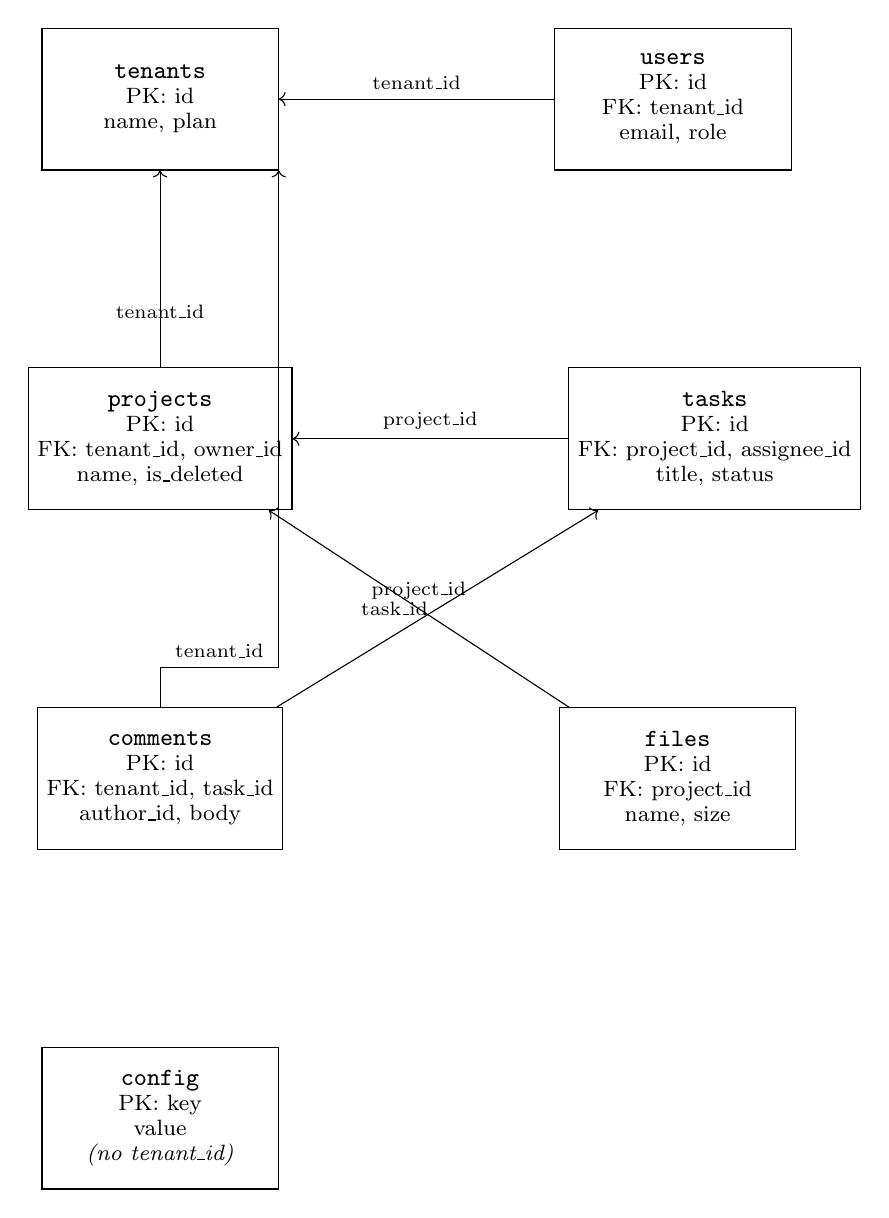
\begin{tikzpicture}[
  entity/.style={rectangle, draw, minimum width=3cm, minimum height=1.8cm,
    align=center, font=\small\ttfamily},
  every edge/.style={draw, -{Stealth[length=6pt]}},
  node distance=2cm and 3cm,
]
  % Entities
  \node[entity] (tenants) {tenants\\[-2pt]\footnotesize\rmfamily PK: id\\[-2pt]\footnotesize\rmfamily name, plan};
  \node[entity, right=3.5cm of tenants] (users) {users\\[-2pt]\footnotesize\rmfamily PK: id\\[-2pt]\footnotesize\rmfamily FK: tenant\_id\\[-2pt]\footnotesize\rmfamily email, role};
  \node[entity, below=2.5cm of tenants] (projects) {projects\\[-2pt]\footnotesize\rmfamily PK: id\\[-2pt]\footnotesize\rmfamily FK: tenant\_id, owner\_id\\[-2pt]\footnotesize\rmfamily name, is\_deleted};
  \node[entity, right=3.5cm of projects] (tasks) {tasks\\[-2pt]\footnotesize\rmfamily PK: id\\[-2pt]\footnotesize\rmfamily FK: project\_id, assignee\_id\\[-2pt]\footnotesize\rmfamily title, status};
  \node[entity, below=2.5cm of projects] (comments) {comments\\[-2pt]\footnotesize\rmfamily PK: id\\[-2pt]\footnotesize\rmfamily FK: tenant\_id, task\_id\\[-2pt]\footnotesize\rmfamily author\_id, body};
  \node[entity, right=3.5cm of comments] (files) {files\\[-2pt]\footnotesize\rmfamily PK: id\\[-2pt]\footnotesize\rmfamily FK: project\_id\\[-2pt]\footnotesize\rmfamily name, size};
  \node[entity, below=2.5cm of comments] (config) {config\\[-2pt]\footnotesize\rmfamily PK: key\\[-2pt]\footnotesize\rmfamily value\\[-2pt]\footnotesize\rmfamily\itshape (no tenant\_id)};

  % Relationships
  \draw[->] (users) -- node[above,font=\scriptsize\rmfamily]{tenant\_id} (tenants);
  \draw[->] (projects.north) -- ++(0,0.5) -| node[near start,above,font=\scriptsize\rmfamily]{tenant\_id} (tenants.south);
  \draw[->] (tasks) -- node[above,font=\scriptsize\rmfamily]{project\_id} (projects);
  \draw[->] (comments.north) -- ++(0,0.5) -| node[near start,above,font=\scriptsize\rmfamily]{tenant\_id} (tenants.south east);
  \draw[->] (comments) -- node[left,font=\scriptsize\rmfamily]{task\_id} (tasks);
  \draw[->] (files) -- node[above,font=\scriptsize\rmfamily]{project\_id} (projects);
\end{tikzpicture}
\caption{Running example: multi-tenant SaaS schema. Tables \texttt{users},
\texttt{projects}, and \texttt{comments} carry \texttt{tenant\_id} directly.
Tables \texttt{tasks} and \texttt{files} inherit tenant context via FK to
\texttt{projects}. Table \texttt{config} is global (no \texttt{tenant\_id}).}
\label{fig:er-diagram}
\end{figure}

% ============================================================
\section{Introduction \& Motivation}
\label{sec:introduction}
% ============================================================

\subsection{The Problem: Arbitrary RLS Is Undecidable}

PostgreSQL Row-Level Security allows attaching arbitrary SQL predicates to
tables via \texttt{CREATE POLICY}. These predicates execute as part of every
query, filtering rows according to security rules. The mechanism is powerful:
any boolean SQL expression is a valid RLS predicate.

This power is also the fundamental problem. SQL is Turing-complete. An RLS
predicate may invoke user-defined functions, reference arbitrary subqueries,
or encode complex recursive logic. As a consequence:

\begin{theorem}[Undecidability of arbitrary RLS]
\label{thm:undecidable}
Given an arbitrary set of RLS policies expressed as SQL predicates, determining
whether a given row is accessible to a given user is undecidable in general.
\end{theorem}

\begin{proof}[Sketch]
Reduce from the halting problem. Encode a Turing machine's transition function
as a PL/pgSQL function invoked within an RLS \texttt{USING} clause. The
predicate returns \texttt{true} if and only if the machine halts. Determining
row accessibility therefore requires solving the halting problem.
\end{proof}

This undecidability means that no tool can, in general:
\begin{itemize}
  \item Prove that tenant isolation holds across all policies
  \item Detect contradictory policies that block all access
  \item Identify redundant policies that can be safely removed
  \item Verify that a policy change preserves the intended access semantics
\end{itemize}

Organizations managing hundreds of tables and dozens of interacting policies
face an intractable verification burden if policies are authored as raw SQL.

\subsection{The Compiler Insight}

The solution is a shift in perspective: \emph{do not analyze arbitrary SQL;
instead, generate SQL from a language where analysis is decidable.}

This is precisely the strategy used by optimizing compilers. A compiler does
not reason about arbitrary machine code. It operates on a structured
intermediate representation (IR) where transformations are provably correct,
then emits machine code as a final step.

Applied to RLS:
\begin{enumerate}
  \item Define a \textbf{domain-specific language} (DSL) with restricted expressiveness.
  \item Perform all \textbf{analysis and optimization} on the DSL's abstract syntax tree.
  \item \textbf{Compile} the DSL deterministically to PostgreSQL \texttt{CREATE POLICY} statements.
\end{enumerate}

RLS becomes a \emph{compilation target}, not an authoring surface. The DSL is
designed so that the properties we care about --- satisfiability, subsumption,
isolation --- are decidable by construction.

\subsection{Relationship to Prior Work}

The algebra draws on five established formalisms, each covering a distinct
aspect of the system:

\textbf{Bonatti et al.'s access-control algebra}~\cite{bonatti2002algebra}.
Bonatti, De Capitani di Vimercati, and Samarati formalized access-control
policies as algebraic objects supporting union (grant), intersection
(restriction), and difference (exception) operations. Our
permissive/restrictive composition directly corresponds to their
grant/restriction operators. The effective access predicate
$(\bigvee\text{ permissive}) \land (\bigwedge\text{ restrictive})$ is an
instance of their composition framework.

\textbf{Lattice theory}. Policies ordered by subsumption form a lattice. The
join ($\sqcup$) corresponds to disjunction of permissive policies; the meet
($\sqcap$) to conjunction of restrictive policies. Redundancy detection
reduces to identifying elements dominated by existing lattice members.

\textbf{SMT solving} (Satisfiability Modulo Theories)~\cite{smtlib,demoura2008z3}.
The atoms of our algebra --- column comparisons with session variables and
literals --- fall within the quantifier-free fragments of linear integer
arithmetic (QF-LIA) and equality with uninterpreted functions (QF-EUF). These
are decidable theories supported by solvers such as Z3 and cvc5. We use SMT to
check clause satisfiability, detect contradictions, and prove tenant isolation.

\textbf{Formal Concept Analysis}~\cite{ganter1999formal} (Ganter \& Wille).
Selectors --- predicates over table metadata --- define a Galois connection
between the power set of tables and the power set of structural attributes.
The closed sets (formal concepts) correspond to natural groupings of tables
sharing common structure, providing a principled foundation for policy
targeting.

\textbf{Galois connections for compiler correctness}~\cite{cousot1977abstract}.
The compilation function from DSL policies to SQL artifacts, paired with the
denotational semantics of each, forms a Galois connection. This structure
provides the framework for stating and proving that compilation preserves the
intended access semantics.

\subsection{Scope and Audience}

This specification covers the \textbf{full lifecycle} of the policy algebra:
\begin{itemize}
  \item \textbf{Definition}: atoms, clauses, policies, selectors, relationship traversal
  \item \textbf{Analysis}: satisfiability, subsumption, redundancy, contradiction, isolation
  \item \textbf{Optimization}: rewrite rules, normal forms, termination
  \item \textbf{Compilation}: deterministic translation to PostgreSQL artifacts
  \item \textbf{Monitoring}: drift detection and reconciliation
\end{itemize}

The intended audience is \textbf{senior engineers} implementing or evaluating
the policy engine, as well as researchers interested in the formal foundations
of database access control.

% ============================================================
\section{Atoms \& Value Sources}
\label{sec:atoms}
% ============================================================

Atoms are the irreducible predicates of the policy algebra. Every policy
ultimately reduces to a boolean combination of atoms, each representing a
single comparison.

\subsection{Value Sources}

A \textbf{value source} produces a scalar value for comparison. The algebra
recognizes four kinds:

\begin{definition}[Value source]
\label{def:value-source}
\begin{lstlisting}[style=bnf]
ValueSource ::= col(name)
              | session(key)
              | lit(v)
              | fn(name, args)
\end{lstlisting}
\end{definition}

Where:
\begin{itemize}
  \item \texttt{col(name)} --- references a column of the table to which the
    policy is attached. The column must exist in the table's schema. Example:
    \texttt{col('tenant\_id')}.
  \item \texttt{session(key)} --- retrieves a runtime session variable via
    PostgreSQL's \texttt{current\_setting(key)}. Example:
    \texttt{session('app.tenant\_id')} compiles to
    \texttt{current\_setting('app.tenant\_id')}.
  \item \texttt{lit(v)} --- a literal constant value: string, integer,
    boolean, or null. Example: \texttt{lit('admin')}, \texttt{lit(42)},
    \texttt{lit(true)}.
  \item \texttt{fn(name, args)} --- a call to a whitelisted, pure,
    deterministic function. The function must be registered in the policy
    engine's function allowlist. Example: \texttt{fn('auth.uid', [])} compiles
    to \texttt{auth.uid()}.
\end{itemize}

\begin{definition}[Value source type]
\label{def:value-source-type}
Each value source has an associated type drawn from
$\{\texttt{text}, \texttt{integer}, \texttt{bigint}, \texttt{uuid},
\texttt{boolean}, \texttt{timestamp}, \texttt{jsonb}\}$.
Type compatibility is enforced at policy definition time, not at compilation.
\end{definition}

\subsection{Atoms}

\begin{definition}[Atom]
\label{def:atom}
An atom is a triple $(\mathit{left}, \mathit{op}, \mathit{right})$ where:
\begin{itemize}
  \item $\mathit{left}$ and $\mathit{right}$ are value sources
  \item $\mathit{op}$ is a comparison operator from the set
    $\{=, \neq, <, >, \leq, \geq, \texttt{IN}, \texttt{NOT IN},
    \texttt{IS NULL}, \texttt{IS NOT NULL}, \texttt{LIKE}, \texttt{NOT LIKE}\}$
\end{itemize}
For unary operators (\texttt{IS NULL}, \texttt{IS NOT NULL}), $\mathit{right}$
is omitted (or equivalently, $\mathit{right} = \texttt{lit(null)}$).
\end{definition}

BNF fragment:
\begin{lstlisting}[style=bnf]
<atom>         ::= <value_source> <binary_op> <value_source>
                 | <value_source> <unary_op>

<binary_op>    ::= "=" | "!=" | "<" | ">" | "<=" | ">="
                 | "IN" | "NOT IN" | "LIKE" | "NOT LIKE"

<unary_op>     ::= "IS NULL" | "IS NOT NULL"

<value_source> ::= "col(" <identifier> ")"
                 | "session(" <string_literal> ")"
                 | "lit(" <literal_value> ")"
                 | "fn(" <identifier> "," "[" <arg_list> "]" ")"
\end{lstlisting}

\textbf{Examples}:

\begin{table}[h]
\centering
\begin{tabular}{ll}
\toprule
Atom & Informal meaning \\
\midrule
\texttt{(col('tenant\_id'), =, session('app.tenant\_id'))} & Row's tenant matches session tenant \\
\texttt{(col('role'), =, lit('admin'))} & User role is admin \\
\texttt{(col('is\_deleted'), =, lit(false))} & Row is not soft-deleted \\
\texttt{(col('status'), IN, lit(['active','pending']))} & Status is active or pending \\
\texttt{(col('deleted\_at'), IS NULL, \_)} & No deletion timestamp \\
\bottomrule
\end{tabular}
\end{table}

\subsection{Atom Normal Form}

To enable comparison and deduplication, atoms are normalized to a canonical form.

\begin{definition}[Atom normal form]
\label{def:atom-normal-form}
An atom is in normal form when:
\begin{enumerate}
  \item \textbf{Column-left ordering}: if exactly one operand is
    \texttt{col(\ldots)}, it appears on the left. If both are columns, they
    are ordered lexicographically by column name.
  \item \textbf{Operator canonicalization}: \texttt{>} is rewritten to
    \texttt{<} (with operands swapped); \texttt{>=} to \texttt{<=};
    \texttt{!=} to \texttt{NOT =}.
  \item \textbf{Literal simplification}: \texttt{lit(true)} in a boolean
    equality is absorbed (e.g., \texttt{col('active') = lit(true)} normalizes
    to \texttt{col('active') IS NOT NULL} only for boolean columns where null
    means false; otherwise left as-is).
\end{enumerate}
\end{definition}

\textbf{Algorithm}: $\texttt{normalize\_atom}(a) \to a'$ applies rules 1--3 in sequence.

\subsection{Atom Equivalence and Subsumption}

\begin{definition}[Atom equivalence]
\label{def:atom-equiv}
Two atoms $a_1$ and $a_2$ are equivalent, written $a_1 \equiv a_2$, if and
only if their normal forms are syntactically identical.
\end{definition}

\begin{definition}[Atom subsumption]
\label{def:atom-subsumption}
Atom $a_1$ subsumes atom $a_2$, written $a_1 \sqsubseteq a_2$, if every row
satisfying $a_2$ also satisfies $a_1$. Equivalently, $a_2 \vdash a_1$ ($a_2$
entails $a_1$).
\end{definition}

Examples of subsumption:
\begin{itemize}
  \item $\texttt{col('x') IS NOT NULL} \sqsubseteq \texttt{col('x') = lit(5)}$
    --- equality implies non-null
  \item $\texttt{col('x') IN lit([1,2,3])} \sqsubseteq \texttt{col('x') IN lit([1,2])}$
    --- subset of IN-list
\end{itemize}

\subsection{Decidability of Atom Satisfiability}

\begin{property}[Decidability]
\label{prop:atom-decidability}
The satisfiability of any finite conjunction of atoms is decidable.
\end{property}

\begin{proof}[Sketch]
Each atom translates to a formula in the quantifier-free theory of linear
integer arithmetic with equality and uninterpreted functions
(QF-LIA $\cup$ QF-EUF). Column references become free variables; session
variables become distinct free variables; literals become constants. The
conjunction of translated atoms is a QF-LIA/EUF formula, which is decidable
by the Nelson-Oppen combination procedure as implemented in SMT solvers.
\end{proof}

% ============================================================
\section{Clauses}
\label{sec:clauses}
% ============================================================

A clause is the fundamental unit of row-level access control: a conjunction of
atoms that must all be satisfied for a row to match.

\subsection{Definition}

\begin{definition}[Clause]
\label{def:clause}
A clause $c$ is a finite set of atoms, interpreted as their conjunction:
\[
c = \{a_1, a_2, \ldots, a_n\} \quad\text{meaning}\quad a_1 \land a_2 \land \cdots \land a_n
\]
The empty clause $\{\}$ is the trivial clause, equivalent to $\top$ (always true).
\end{definition}

BNF fragment:
\begin{lstlisting}[style=bnf]
<clause>    ::= <atom>
              | <atom> "AND" <clause>
\end{lstlisting}

\subsection{Clause Normal Form}

\begin{definition}[Clause normal form]
\label{def:clause-normal-form}
A clause is in normal form when:
\begin{enumerate}
  \item Every constituent atom is in atom normal form (Def.~\ref{def:atom-normal-form}).
  \item Atoms are sorted lexicographically by their normal-form string representation.
  \item Duplicate atoms (by equivalence, Def.~\ref{def:atom-equiv}) are removed.
  \item If any pair of atoms is contradictory, the entire clause is replaced by $\bot$.
\end{enumerate}
\end{definition}

A pair of atoms is contradictory when their conjunction is unsatisfiable.
Common cases detected syntactically:
\begin{itemize}
  \item $\texttt{col}(x) = \texttt{lit}(v_1) \land \texttt{col}(x) = \texttt{lit}(v_2)$ where $v_1 \neq v_2$
  \item $\texttt{col}(x)\ \texttt{IS NULL} \land \texttt{col}(x) = \texttt{lit}(v)$ for any non-null $v$
  \item $\texttt{col}(x) = \texttt{lit}(v) \land \texttt{col}(x) \neq \texttt{lit}(v)$
\end{itemize}

\textbf{Algorithm}: $\texttt{normalize\_clause}(c) \to c'$:

\begin{lstlisting}[style=pseudo]
function normalize_clause(c):
    c' <- {normalize_atom(a) | a in c}
    c' <- deduplicate(c')
    if has_syntactic_contradiction(c'):
        return bot
    return sort(c')
\end{lstlisting}

\subsection{Clause Properties}

\begin{property}[Clause satisfiability]
\label{prop:clause-sat}
A normalized clause $c$ is satisfiable if and only if $c \neq \bot$. For
non-syntactic contradictions, SMT solving (Property~\ref{prop:atom-decidability})
provides a complete decision procedure.
\end{property}

\begin{property}[Clause subsumption]
\label{prop:clause-subsumption}
Clause $c_1$ subsumes clause $c_2$, written $c_1 \sqsubseteq c_2$, if and
only if every atom in $c_1$ is subsumed by some atom in $c_2$ or implied by
the conjunction of atoms in $c_2$.
\end{property}

A sufficient syntactic check: $c_1 \subseteq c_2$ (every atom in $c_1$
appears in $c_2$) implies $c_2 \sqsubseteq c_1$. Note the direction: more
atoms means more constraints, hence fewer matching rows, hence the clause
with more atoms is subsumed by (is less permissive than) the clause with
fewer atoms.

More precisely: if $c_1 \subseteq c_2$ then
$\denote{c_2} \subseteq \denote{c_1}$ (the denotation of $c_2$ is a subset
of the denotation of $c_1$), so $c_1 \sqsubseteq c_2$ in the ``more
permissive'' ordering.

\begin{property}[Idempotence]
\label{prop:idempotence}
For any clause $c$: $c \land c = c$.
\end{property}

\begin{proof}
Clause conjunction merges atom sets. Deduplication yields the original set.
\end{proof}

\textbf{Example}:
\begin{lstlisting}[style=dsl]
c1 = {col('tenant_id') = session('app.tenant_id')}
c2 = {col('tenant_id') = session('app.tenant_id'),
      col('role') = lit('editor')}

c1 subsumes c2:  c1 (*@$\subseteq$@*) c2, so (*@$\denote{c_2} \subseteq \denote{c_1}$@*)
    c1 is more permissive (fewer constraints, more rows match)
\end{lstlisting}

% ============================================================
\section{Policies}
\label{sec:policies}
% ============================================================

A policy is a named, typed collection of clauses that applies to specific SQL
commands on tables selected by a selector predicate.

\subsection{Definition}

\begin{definition}[Policy]
\label{def:policy}
A policy is a 5-tuple:
\[
p = (\mathit{name},\ \mathit{type},\ \mathit{commands},\ \mathit{selector},\ \mathit{clauses})
\]
Where:
\begin{itemize}
  \item $\mathit{name} \in \mathrm{String}$ --- a unique identifier for the policy
  \item $\mathit{type} \in \{\texttt{permissive}, \texttt{restrictive}\}$
  \item $\mathit{commands} \subseteq \{\texttt{SELECT}, \texttt{INSERT}, \texttt{UPDATE}, \texttt{DELETE}\}$, non-empty
  \item $\mathit{selector}$ --- a selector predicate (Section~\ref{sec:selectors}) determining which tables this policy applies to
  \item $\mathit{clauses} = \{c_1, c_2, \ldots, c_n\}$ --- a non-empty finite set of clauses
\end{itemize}
\end{definition}

BNF fragment:
\begin{lstlisting}[style=bnf]
<policy>          ::= "POLICY" <identifier>
                      <policy_type>
                      <command_list>
                      <selector_clause>
                      <clause_block>

<policy_type>     ::= "PERMISSIVE" | "RESTRICTIVE"
<command_list>    ::= "FOR" <command> ("," <command>)*
<command>         ::= "SELECT" | "INSERT" | "UPDATE" | "DELETE"
<selector_clause> ::= "SELECTOR" <selector>
<clause_block>    ::= "CLAUSE" <clause> ("OR" "CLAUSE" <clause>)*
\end{lstlisting}

\subsection{Policy Denotation}

\begin{definition}[Policy denotation]
\label{def:policy-denotation}
The denotation of a policy $p$ is the disjunction of its clauses:
\[
\denote{p} = \denote{c_1} \lor \denote{c_2} \lor \cdots \lor \denote{c_n}
\]
A row satisfies a policy if it satisfies \emph{any} of the policy's clauses.
\end{definition}

\subsection{USING vs WITH CHECK}

For write commands (\texttt{INSERT}, \texttt{UPDATE}, \texttt{DELETE}),
PostgreSQL~\cite{postgresql-rls} distinguishes:
\begin{itemize}
  \item \textbf{USING}: filters which existing rows are visible (relevant for
    \texttt{UPDATE}, \texttt{DELETE}, and \texttt{SELECT} within an
    \texttt{UPDATE}/\texttt{DELETE})
  \item \textbf{WITH CHECK}: validates new or modified rows (relevant for
    \texttt{INSERT} and the new values in \texttt{UPDATE})
\end{itemize}

In this algebra, each policy carries a single set of clauses that serves as
both \texttt{USING} and \texttt{WITH CHECK} by default. A policy may
optionally specify separate \texttt{with\_check\_clauses} when the
write-validation predicate differs from the read-visibility predicate.

\begin{definition}[Policy with distinct check]
\label{def:policy-distinct-check}
An extended policy is a 6-tuple
$(\mathit{name}, \mathit{type}, \mathit{commands}, \mathit{selector},
\mathit{using\_clauses}, \mathit{check\_clauses})$ where
$\mathit{check\_clauses}$ defaults to $\mathit{using\_clauses}$ if unspecified.
\end{definition}

\subsection{Example: Tenant Isolation Policy}

\begin{lstlisting}[style=dsl]
POLICY tenant_isolation
  PERMISSIVE
  FOR SELECT, INSERT, UPDATE, DELETE
  SELECTOR has_column('tenant_id')
  CLAUSE col('tenant_id') = session('app.tenant_id')
\end{lstlisting}

This defines a single permissive policy with one clause containing one atom.
The selector \texttt{has\_column('tenant\_id')} causes it to apply to
\texttt{users}, \texttt{projects}, and \texttt{comments} in our running
example, but \emph{not} to \texttt{tasks}, \texttt{files} (no direct
\texttt{tenant\_id}), or \texttt{config} (global table).

% ============================================================
\section{Composition --- The Policy Lattice}
\label{sec:composition}
% ============================================================

This section defines how multiple policies on a single table combine to
produce an effective access predicate. The composition rules follow
PostgreSQL's native semantics and correspond to Bonatti et
al.'s~\cite{bonatti2002algebra} access-control algebra.

\subsection{Table Policy Set}

\begin{definition}[Table policy set]
\label{def:table-policy-set}
For a given table $T$ and command $\CMD$, the \emph{table policy set} is the
set of all policies whose selector matches $T$ and whose command set includes
$\CMD$:
\[
\Pol(T, \CMD) = \{p \mid \mathrm{match}(p.\mathit{selector}, T) \land \CMD \in p.\mathit{commands}\}
\]
This set partitions into permissive and restrictive subsets:
\begin{align*}
\Perm(T, \CMD) &= \{p \in \Pol(T, \CMD) \mid p.\mathit{type} = \texttt{permissive}\} \\
\Rest(T, \CMD) &= \{p \in \Pol(T, \CMD) \mid p.\mathit{type} = \texttt{restrictive}\}
\end{align*}
\end{definition}

\subsection{Effective Access Predicate}

\begin{definition}[Effective access predicate]
\label{def:effective}
The effective access predicate for table $T$ under command $\CMD$ is:
\[
\Eff(T, \CMD) = \left(\bigvee_{p \in \Perm} \denote{p}\right) \land \left(\bigwedge_{r \in \Rest} \denote{r}\right)
\]
Expanding policy denotations:
\[
\Eff(T, \CMD) = \left(\bigvee_{p \in \Perm} \bigvee_{c \in p.\mathit{clauses}} \denote{c}\right) \land \left(\bigwedge_{r \in \Rest} \bigvee_{c \in r.\mathit{clauses}} \denote{c}\right)
\]
\end{definition}

\subsection{Default Deny}

\begin{definition}[Default deny]
\label{def:default-deny}
If $\Perm(T, \CMD) = \emptyset$ (no permissive policies apply), then
$\Eff(T, \CMD) = \bot$. No rows are accessible.
\end{definition}

This follows from the convention that an empty disjunction is $\bot$.
Restrictive policies alone cannot grant access --- they can only further
restrict access already granted by permissive policies.

\subsection{Connection to Bonatti's Algebra}

Bonatti et al.~\cite{bonatti2002algebra} define an access-control algebra with
three operators:

\begin{table}[h]
\centering
\begin{tabular}{lll}
\toprule
Bonatti operator & This algebra & Effect \\
\midrule
$+$ (grant/union) & Permissive policy disjunction & Expands accessible rows \\
$\&$ (restriction/intersection) & Restrictive policy conjunction & Narrows accessible rows \\
$-$ (exception/difference) & Not directly supported & Would allow row-level exceptions \\
\bottomrule
\end{tabular}
\end{table}

The effective predicate formula maps directly:
\[
\Eff = \left(+_{p \in \Perm} \denote{p}\right)\ \&\ \left(\&_{r \in \Rest} \denote{r}\right)
\]

The absence of the exception operator ($-$) is deliberate: exceptions
complicate analysis and are not needed for the patterns targeted by this
algebra (tenant isolation, role-based access, soft-delete filtering).

\subsection{Monotonicity Properties}

\begin{property}[Monotonicity of permissive extension]
\label{prop:perm-mono}
Adding a permissive policy to $\Perm$ can only increase (or maintain) the set
of accessible rows.
\end{property}

\begin{proof}
Let $\Perm' = \Perm \cup \{p_{\mathrm{new}}\}$. Then:
\[
\bigvee_{p \in \Perm'} \denote{p} = \left(\bigvee_{p \in \Perm} \denote{p}\right) \lor \denote{p_{\mathrm{new}}} \supseteq \bigvee_{p \in \Perm} \denote{p}
\]
Since $A \lor B \supseteq A$ for any predicates $A$, $B$ (in terms of
satisfying rows), the effective predicate's permissive component can only grow.
\end{proof}

\begin{property}[Anti-monotonicity of restrictive extension]
\label{prop:rest-anti-mono}
Adding a restrictive policy to $\Rest$ can only decrease (or maintain) the set
of accessible rows.
\end{property}

\begin{proof}
Let $\Rest' = \Rest \cup \{r_{\mathrm{new}}\}$. Then:
\[
\bigwedge_{r \in \Rest'} \denote{r} = \left(\bigwedge_{r \in \Rest} \denote{r}\right) \land \denote{r_{\mathrm{new}}} \subseteq \bigwedge_{r \in \Rest} \denote{r}
\]
Since $A \land B \subseteq A$ for any predicates $A$, $B$.
\end{proof}

\subsection{Policy Subsumption and Redundancy}

\begin{definition}[Policy subsumption]
\label{def:policy-subsumption}
Permissive policy $p_1$ subsumes permissive policy $p_2$, written
$p_1 \sqsupseteq p_2$, if:
\[
\denote{p_2} \subseteq \denote{p_1}
\]
That is, every row accessible under $p_2$ is also accessible under $p_1$.
\end{definition}

\begin{definition}[Policy redundancy]
\label{def:policy-redundancy}
A policy $p$ in policy set $S$ is \emph{redundant} if removing it does not
change the effective access predicate:
\[
\Eff_S(T, \CMD) = \Eff_{S \setminus \{p\}}(T, \CMD)
\]
\end{definition}

\begin{lemma}[Subsumed permissive policy is redundant]
\label{lem:subsumed-redundant}
If permissive policy $p_2$ is subsumed by another permissive policy
$p_1 \in \Perm$, then $p_2$ is redundant in $\Perm$.
\end{lemma}

\begin{proof}[Sketch]
Since $\denote{p_2} \subseteq \denote{p_1}$:
\[
\bigvee_{p \in \Perm} \denote{p} = \denote{p_1} \lor \denote{p_2} \lor \bigvee_{p \in \Perm \setminus \{p_1, p_2\}} \denote{p}
= \denote{p_1} \lor \bigvee_{p \in \Perm \setminus \{p_1, p_2\}} \denote{p}
\]
by absorption ($A \lor B = A$ when $B \subseteq A$). Removing $p_2$ leaves the
disjunction unchanged.
\end{proof}

A sufficient syntactic condition for policy subsumption: $p_1 \sqsupseteq p_2$
if for every clause $c_2 \in p_2.\mathit{clauses}$, there exists a clause
$c_1 \in p_1.\mathit{clauses}$ such that $c_1 \sqsubseteq c_2$ (i.e., $c_1$
has a subset of $c_2$'s atoms, so $c_1$ is at least as permissive).

\subsection{Worked Example}

Consider two policies on the \texttt{projects} table for \texttt{SELECT}:

\begin{lstlisting}[style=dsl]
POLICY tenant_isolation          POLICY soft_delete
  PERMISSIVE                       RESTRICTIVE
  FOR SELECT                       FOR SELECT
  SELECTOR has_column('tenant_id') SELECTOR has_column('is_deleted')
  CLAUSE                           CLAUSE
    col('tenant_id') =               col('is_deleted') = lit(false)
      session('app.tenant_id')
\end{lstlisting}

Both selectors match \texttt{projects} (which has both \texttt{tenant\_id} and
\texttt{is\_deleted}).

Partition: $\Perm = \{\text{tenant\_isolation}\}$, $\Rest = \{\text{soft\_delete}\}$.

Effective predicate:
\begin{align*}
\Eff(\texttt{projects}, \texttt{SELECT})
  &= \denote{\text{tenant\_isolation}} \land \denote{\text{soft\_delete}} \\
  &= (\texttt{col('tenant\_id')} = \texttt{session('app.tenant\_id')}) \\
  &\quad \land (\texttt{col('is\_deleted')} = \texttt{lit(false)})
\end{align*}

A \texttt{SELECT} on \texttt{projects} returns only rows where the tenant
matches \emph{and} the row is not soft-deleted.

% ============================================================
\section{Selectors \& Table Matching}
\label{sec:selectors}
% ============================================================

Selectors decouple policies from specific table names. Instead of enumerating
tables, a policy declares structural criteria. Tables matching those criteria
receive the policy automatically --- including tables added in the future.

\subsection{Selector Predicates}

\begin{definition}[Selector]
\label{def:selector}
A selector is a predicate over table metadata, constructed from the following grammar:
\begin{lstlisting}[style=bnf]
<selector>       ::= <base_selector>
                    | <selector> "AND" <selector>
                    | <selector> "OR" <selector>
                    | "NOT" <selector>
                    | "(" <selector> ")"
                    | "ALL"

<base_selector>  ::= "has_column(" <identifier> ("," <type>)? ")"
                    | "in_schema(" <identifier> ")"
                    | "named(" <pattern> ")"
                    | "tagged(" <tag> ")"
\end{lstlisting}
\end{definition}

Where:
\begin{itemize}
  \item \texttt{has\_column(name, type?)} --- matches tables that have a column
    with the given name, optionally restricted to a specific type.
  \item \texttt{in\_schema(s)} --- matches tables in the specified PostgreSQL schema.
  \item \texttt{named(pat)} --- matches tables whose name matches the given
    pattern (SQL \texttt{LIKE} syntax).
  \item \texttt{tagged(t)} --- matches tables that carry the specified metadata tag.
  \item \texttt{ALL} --- matches every table in the governed set.
\end{itemize}

\subsection{Table Metadata Context}

\begin{definition}[Table metadata context]
\label{def:metadata-context}
The metadata context $M$ is the set of structural facts about all tables in
the governed database, extracted from \texttt{pg\_catalog}:
\[
M = \{ (\mathit{table\_name}, \mathit{schema\_name}, \mathit{columns}, \mathit{tags}) \mid \text{table} \in \text{governed\_tables} \}
\]
Where $\mathit{columns}$ is a set of $(\mathit{column\_name}, \mathit{column\_type})$ pairs,
and $\mathit{tags}$ is a set of string labels.
\end{definition}

\subsection{Matching Function}

\begin{definition}[Selector matching]
\label{def:selector-matching}
The function $\mathrm{match}$ evaluates a selector against the metadata context
to produce a set of matching tables:
\begin{align*}
\mathrm{match} &: \mathrm{Selector} \times M \to \mathcal{P}(\mathrm{Table}) \\
\mathrm{match}(\texttt{has\_column}(n, t), M) &= \{T \in M \mid (n, t') \in T.\mathit{columns} \land (t = \_ \lor t = t')\} \\
\mathrm{match}(\texttt{in\_schema}(s), M) &= \{T \in M \mid T.\mathit{schema} = s\} \\
\mathrm{match}(\texttt{named}(\mathit{pat}), M) &= \{T \in M \mid T.\mathit{name}\ \texttt{LIKE}\ \mathit{pat}\} \\
\mathrm{match}(\texttt{tagged}(t), M) &= \{T \in M \mid t \in T.\mathit{tags}\} \\
\mathrm{match}(s_1\ \texttt{AND}\ s_2, M) &= \mathrm{match}(s_1, M) \cap \mathrm{match}(s_2, M) \\
\mathrm{match}(s_1\ \texttt{OR}\ s_2, M) &= \mathrm{match}(s_1, M) \cup \mathrm{match}(s_2, M) \\
\mathrm{match}(\texttt{NOT}\ s, M) &= M \setminus \mathrm{match}(s, M) \\
\mathrm{match}(\texttt{ALL}, M) &= M
\end{align*}
\end{definition}

\textbf{Example}: In our running schema:
\begin{align*}
\mathrm{match}(\texttt{has\_column('tenant\_id')}, M) &= \{\texttt{users}, \texttt{projects}, \texttt{comments}\} \\
\mathrm{match}(\texttt{has\_column('is\_deleted')}, M) &= \{\texttt{projects}\} \\
\mathrm{match}(\texttt{ALL}, M) &= \{\texttt{users}, \texttt{projects}, \texttt{tasks}, \texttt{comments}, \texttt{files}, \texttt{config}\}
\end{align*}

\subsection{Connection to Formal Concept Analysis}

The selector mechanism admits a natural interpretation in Formal Concept
Analysis (FCA)~\cite{ganter1999formal}:
\begin{itemize}
  \item \textbf{Objects} = the set of governed tables
  \item \textbf{Attributes} = structural properties (has column X, in schema Y, etc.)
  \item \textbf{Incidence relation} = table $T$ has attribute $A$ iff the corresponding
    base selector is satisfied
\end{itemize}

A \textbf{formal concept} is a pair $(\mathit{extent}, \mathit{intent})$ where:
\begin{itemize}
  \item $\mathit{extent}$ is a maximal set of tables sharing all attributes in $\mathit{intent}$
  \item $\mathit{intent}$ is a maximal set of attributes shared by all tables in $\mathit{extent}$
\end{itemize}

The closure operators forming the Galois connection between $\mathcal{P}(\text{Tables})$
and $\mathcal{P}(\text{Attributes})$ are:
\begin{align*}
\alpha(T_{\mathrm{set}}) &= \{a \in \text{Attributes} \mid \forall T \in T_{\mathrm{set}}: T \text{ has } a\} \\
\beta(A_{\mathrm{set}}) &= \{T \in \text{Tables} \mid \forall a \in A_{\mathrm{set}}: T \text{ has } a\}
\end{align*}

A selector $s$ defines an attribute set, and $\mathrm{match}(s, M)$ computes
$\beta$ applied to that set. This means selectors are computing extents of
(possibly non-closed) attribute sets. The formal concepts represent the natural
``policy groups'' --- maximal clusters of tables sharing structural properties.

\subsection{Selector Monotonicity}

\begin{property}[Selector monotonicity]
\label{prop:selector-mono}
For a fixed selector $s$, if a new table $T_{\mathrm{new}}$ is added to the
governed database and $\mathrm{match}(s, M)$ included tables
$T_1, \ldots, T_k$, then
$\mathrm{match}(s, M \cup \{T_{\mathrm{new}}\}) \supseteq \{T_1, \ldots, T_k\}$.
\end{property}

\begin{proof}
Selector evaluation depends only on each table's own metadata. Adding a new
table cannot change the metadata of existing tables, so existing matches are
preserved. The new table either matches (expanding the set) or doesn't
(leaving it unchanged).
\end{proof}

This property ensures that policy coverage is stable under schema evolution:
existing protections are never silently dropped when new tables are added.

% ============================================================
\section{Relationship Traversal}
\label{sec:traversal}
% ============================================================

Some tables do not carry a direct \texttt{tenant\_id} column but inherit
tenant context through foreign-key relationships. The \texttt{tasks} table in
our running example has no \texttt{tenant\_id} but references \texttt{projects},
which does. Relationship traversal allows policies to express this indirect
access pattern.

\subsection{Declared Relationships}

\begin{definition}[Relationship]
\label{def:relationship}
A declared relationship is a 4-tuple:
\[
\texttt{rel}(\mathit{source\_table}, \mathit{source\_col}, \mathit{target\_table}, \mathit{target\_col})
\]
Where $\mathit{source\_table}.\mathit{source\_col}$ is a foreign key
referencing $\mathit{target\_table}.\mathit{target\_col}$.
\end{definition}

\textbf{Example}: $\texttt{rel(tasks, project\_id, projects, id)}$ declares
that \texttt{tasks.project\_id} references \texttt{projects.id}.

Relationships are declared explicitly in the policy configuration, not inferred
from database constraints. This ensures that only intentional access paths are
used for policy traversal.

\subsection{Traversal Atoms}

\begin{definition}[Traversal atom]
\label{def:traversal-atom}
A traversal atom extends the atom grammar with an existential subquery:
\begin{lstlisting}[style=bnf]
<traversal_atom> ::= "exists(" <relationship> "," <clause> ")"
\end{lstlisting}
Semantics: $\texttt{exists}(\texttt{rel}(S, sc, T, tc), \mathit{clause})$ is
satisfied for a row $r$ of table $S$ if there exists a row $r'$ in table $T$
such that $r.sc = r'.tc$ and $\mathit{clause}(r')$ holds.
\end{definition}

\textbf{Example}:
\begin{lstlisting}[style=dsl]
exists(
  rel(tasks, project_id, projects, id),
  {col('tenant_id') = session('app.tenant_id')}
)
\end{lstlisting}

This atom on the \texttt{tasks} table checks: ``there exists a project row
whose \texttt{id} matches this task's \texttt{project\_id} and whose
\texttt{tenant\_id} matches the session tenant.'' This provides tenant
isolation for \texttt{tasks} through the relationship to \texttt{projects}.

Extended BNF:
\begin{lstlisting}[style=bnf]
<atom> ::= <value_source> <binary_op> <value_source>
         | <value_source> <unary_op>
         | <traversal_atom>

<traversal_atom> ::= "exists(" <relationship> "," <clause> ")"

<relationship>   ::= "rel(" <identifier> "," <identifier> ","
                            <identifier> "," <identifier> ")"
\end{lstlisting}

\subsection{Traversal Depth}

\begin{definition}[Traversal depth]
\label{def:traversal-depth}
The \emph{depth} of an atom is defined recursively:
\begin{align*}
\mathrm{depth}(\mathit{value\_source}\ \mathit{op}\ \mathit{value\_source}) &= 0 \\
\mathrm{depth}(\mathit{value\_source}\ \mathit{unary\_op}) &= 0 \\
\mathrm{depth}(\texttt{exists}(\mathit{rel}, \mathit{clause})) &= 1 + \max(\{\mathrm{depth}(a) \mid a \in \mathit{clause}\})
\end{align*}
The depth of a clause is $\max(\{\mathrm{depth}(a) \mid a \in \mathit{clause}\})$.
\end{definition}

\begin{definition}[Maximum traversal depth]
\label{def:max-depth}
The policy engine enforces a global maximum traversal depth $D$ (default $D = 2$).
Any atom with $\mathrm{depth}(a) > D$ is rejected at definition time.
\end{definition}

\subsection{Properties}

\begin{property}[Bounded compilation]
\label{prop:bounded-compilation}
A traversal atom of depth $d$ compiles to at most $d$ nested \texttt{EXISTS}
subqueries. With maximum depth $D$, the compiled SQL has at most $D$ levels
of nesting.
\end{property}

\begin{proof}
By structural induction on the traversal atom. Base case: a non-traversal
atom compiles to a flat SQL expression (depth 0). Inductive step:
$\texttt{exists}(\mathit{rel}, \mathit{clause})$ compiles to
\texttt{EXISTS (SELECT 1 FROM T WHERE join\_cond AND compile(clause))},
adding one nesting level to whatever $\texttt{compile}(\mathit{clause})$
produces.
\end{proof}

\begin{property}[No recursive traversal]
\label{prop:no-recursive}
The algebra does not support recursive relationship traversal. Hierarchical
access patterns (e.g., org trees) require pre-computed closure tables rather
than recursive policy expressions.
\end{property}

This restriction is essential for decidability. Recursive traversal would
require fixpoint computation, pushing the algebra beyond the decidable fragment.

\subsection{Example: Tenant Isolation via Traversal}

For \texttt{tasks} (no \texttt{tenant\_id}) and \texttt{files} (no \texttt{tenant\_id}):

\begin{lstlisting}[style=dsl]
POLICY tenant_isolation_via_project
  PERMISSIVE
  FOR SELECT, INSERT, UPDATE, DELETE
  SELECTOR named('tasks') OR named('files')
  CLAUSE
    exists(
      rel(_, project_id, projects, id),
      {col('tenant_id') = session('app.tenant_id')}
    )
\end{lstlisting}

When applied to \texttt{tasks}, the compiled SQL becomes:

\begin{lstlisting}[style=sql]
CREATE POLICY tenant_isolation_via_project ON tasks
  USING (EXISTS (
    SELECT 1 FROM projects
    WHERE projects.id = tasks.project_id
      AND projects.tenant_id = current_setting('app.tenant_id')
  ));
\end{lstlisting}

% ============================================================
\section{Analysis}
\label{sec:analysis}
% ============================================================

Because the algebra is decidable, policies can be analyzed \emph{at design
time}, before any SQL is generated or executed. This section defines the key
analysis operations: satisfiability, subsumption, redundancy, contradiction,
and tenant isolation proofs.

\subsection{Satisfiability}

Satisfiability asks: ``Can this clause/policy ever match any row?'' An
unsatisfiable clause is a contradiction --- a bug in the policy definition.

\subsubsection{SMT Encoding}

Each atom is encoded as an SMT formula in the combined theory
QF-LIA $\cup$ QF-EUF:

\begin{lstlisting}[style=pseudo]
function encode_atom(a) -> SMT formula:
    match a:
        (col(x), =, col(y))        -> x_var = y_var
        (col(x), =, session(k))    -> x_var = k_var
        (col(x), =, lit(v))        -> x_var = v_const
        (col(x), !=, lit(v))       -> x_var != v_const
        (col(x), <, lit(v))        -> x_var < v_const
        (col(x), IN, lit([v1..]))  -> x_var = v1 | ... | x_var = vn
        (col(x), IS NULL, _)       -> x_null = true
        (col(x), IS NOT NULL, _)   -> x_null = false
        exists(rel, clause)         -> encode_traversal(rel, clause)

function encode_clause(c) -> SMT formula:
    return conjunction of encode_atom(a) for a in c

function encode_traversal(rel(S, sc, T, tc), clause):
    target_vars <- fresh_vars(T)
    join_cond   <- sc_var = target_vars[tc]
    return exists target_vars: join_cond and
           encode_clause(clause)[T -> target_vars]
\end{lstlisting}

The satisfiability check: submit the formula to an SMT solver. If the solver
returns \texttt{UNSAT}, the clause is a contradiction.

\subsubsection{Pseudocode}

\begin{lstlisting}[style=pseudo]
function check_satisfiability(clause c) -> {SAT, UNSAT, UNKNOWN}:
    c' <- normalize_clause(c)
    if c' = bot:
        return UNSAT        -- Syntactic contradiction detected
    phi <- encode_clause(c')
    result <- smt_solve(phi, timeout=5s)
    return result
\end{lstlisting}

\subsubsection{Example}

Consider the clause: $\{\texttt{col('role')} = \texttt{lit('admin')},\
\texttt{col('role')} = \texttt{lit('viewer')}\}$.

After normalization, syntactic contradiction detection finds two equality atoms
on the same column with different literal values. The clause reduces to $\bot$
without needing the SMT solver.

For a subtler case: $\{\texttt{col('age')} > \texttt{lit(65)},\
\texttt{col('age')} < \texttt{lit(18)}\}$. Syntactic checks may not catch
this. The SMT encoding produces:
\[
\mathit{age\_var} > 65 \land \mathit{age\_var} < 18
\]
The solver returns \texttt{UNSAT}: no integer satisfies both constraints.

\subsection{Subsumption}

Subsumption determines whether one policy's access grant is entirely contained
within another's.

\begin{definition}[Policy subsumption via clauses]
\label{def:policy-subsumption-clauses}
Permissive policy $p_1$ subsumes permissive policy $p_2$, written
$p_1 \sqsupseteq p_2$, if:
\[
\forall c_2 \in p_2.\mathit{clauses},\ \exists c_1 \in p_1.\mathit{clauses}: c_1 \sqsubseteq c_2
\]
That is, every clause of $p_2$ is subsumed by some clause of $p_1$.
\end{definition}

\textbf{Algorithm}:

\begin{lstlisting}[style=pseudo]
function check_subsumption(p1, p2) -> bool:
    for each c2 in p2.clauses:
        found <- false
        for each c1 in p1.clauses:
            if clause_subsumes(c1, c2):
                found <- true
                break
        if not found:
            return false
    return true

function clause_subsumes(c1, c2) -> bool:
    -- Syntactic check: c1's atoms are a subset of c2's
    if atoms(c1) is subset of atoms(c2):
        return true
    -- Semantic check: ask SMT if c2 entails c1
    phi <- encode_clause(c2) and not encode_clause(c1)
    return smt_solve(phi) = UNSAT
\end{lstlisting}

\subsection{Redundancy}

\begin{definition}[Redundancy]
\label{def:redundancy}
Policy $p$ is redundant in policy set $S$ if:
\[
\Eff_S(T, \CMD) \equiv \Eff_{S \setminus \{p\}}(T, \CMD)
\]
\end{definition}

\textbf{Algorithm}:

\begin{lstlisting}[style=pseudo]
function check_redundancy(p, S, T, CMD) -> bool:
    if p.type = permissive:
        P_others <- P(T, CMD) \ {p}
        for each c in p.clauses:
            subsumed <- false
            for each p' in P_others:
                for each c' in p'.clauses:
                    if clause_subsumes(c', c):
                        subsumed <- true; break
                if subsumed: break
            if not subsumed:
                return false
        return true
    else:  -- restrictive
        phi_perm <- encode_permissive_disjunction(P(T, CMD))
        phi_p    <- encode_policy(p)
        phi      <- phi_perm and not phi_p
        return smt_solve(phi) = UNSAT
\end{lstlisting}

\subsection{Contradiction}

\begin{definition}[Contradiction]
\label{def:contradiction}
The effective access predicate for table $T$ under command $\CMD$ is
\emph{contradictory} if it is unsatisfiable:
\[
\Eff(T, \CMD) = \bot
\]
This means no rows are ever accessible --- likely a policy authoring error.
\end{definition}

\textbf{Algorithm}:

\begin{lstlisting}[style=pseudo]
function check_contradiction(T, CMD, S) -> bool:
    phi <- encode(effective(T, CMD))
    return smt_solve(phi) = UNSAT
\end{lstlisting}

\textbf{Example}: If the only permissive policy on \texttt{projects} requires
$\texttt{col('role')} = \texttt{lit('admin')}$ and the only restrictive policy
requires $\texttt{col('role')} = \texttt{lit('viewer')}$, the effective predicate is:
\[
\texttt{col('role')} = \texttt{lit('admin')} \land \texttt{col('role')} = \texttt{lit('viewer')}
\]
This is unsatisfiable. The analysis flags a contradiction.

\subsection{Tenant Isolation Proof}

The most important analysis: proving that tenant data is properly isolated.
The question is: \emph{can any session ever access a row belonging to a
different tenant?}

\subsubsection{Formal Statement}

\begin{definition}[Tenant isolation]
\label{def:tenant-isolation}
Table $T$ satisfies tenant isolation if there is no row $r$ and two distinct
sessions $s_1 \neq s_2$ (differing in \texttt{app.tenant\_id}) such that both
sessions can access $r$:
\[
\lnot \exists\, r, s_1, s_2:\
s_1.\mathit{tenant\_id} \neq s_2.\mathit{tenant\_id}
\land \Eff(T, \CMD)[s \mapsto s_1](r)
\land \Eff(T, \CMD)[s \mapsto s_2](r)
\]
If this formula is \textbf{unsatisfiable}, tenant isolation holds.
\end{definition}

\subsubsection{SMT Encoding}

\begin{lstlisting}[style=pseudo]
function prove_tenant_isolation(T, CMD, S)
    -> {PROVEN, FAILED, UNKNOWN}:
    s1_vars <- fresh_session_vars("s1")
    s2_vars <- fresh_session_vars("s2")
    row_vars <- fresh_row_vars(T)

    phi_diff <- s1_vars['app.tenant_id']
                != s2_vars['app.tenant_id']
    phi_eff1 <- encode(effective(T, CMD))
                [session -> s1_vars, row -> row_vars]
    phi_eff2 <- encode(effective(T, CMD))
                [session -> s2_vars, row -> row_vars]

    phi <- phi_diff and phi_eff1 and phi_eff2

    result <- smt_solve(phi)
    if result = UNSAT:
        return PROVEN
    else if result = SAT:
        return FAILED
    else:
        return UNKNOWN
\end{lstlisting}

\subsubsection{Sufficient Condition}

\begin{theorem}[Sufficient condition for tenant isolation]
\label{thm:tenant-isolation}
If every permissive clause for table $T$ contains the atom
$\texttt{col('tenant\_id')} = \texttt{session('app.tenant\_id')}$ (directly
or via a depth-1 traversal to a table with such a clause), then tenant
isolation holds for $T$.
\end{theorem}

\begin{proof}[Sketch]
Suppose two sessions $s_1$ and $s_2$ with different tenant IDs both access row
$r$. Each must satisfy at least one permissive clause (by default deny). Every
permissive clause requires the row's \texttt{tenant\_id} (direct or via
traversal) to equal the session's \texttt{app.tenant\_id}. So:
\begin{align*}
r.\mathit{tenant\_id} &= s_1.\texttt{app.tenant\_id} \\
r.\mathit{tenant\_id} &= s_2.\texttt{app.tenant\_id}
\end{align*}
Therefore $s_1.\texttt{app.tenant\_id} = s_2.\texttt{app.tenant\_id}$,
contradicting the assumption that they differ.
\end{proof}

% ============================================================
\section{Optimization \& Rewrite Rules}
\label{sec:optimization}
% ============================================================

The policy engine applies rewrite rules to simplify policies before
compilation. Each rule preserves the denotation (semantic equivalence) while
reducing syntactic complexity.

\subsection{Rewrite Rules}

\textbf{Rule 1: Idempotence.}
\[
a \land a = a
\]
Duplicate atoms within a clause are removed.

\emph{Example}: $\{\texttt{col('x')}=\texttt{lit(1)}, \texttt{col('x')}=\texttt{lit(1)}\} \to \{\texttt{col('x')}=\texttt{lit(1)}\}$.

\textbf{Rule 2: Absorption.}
\[
c_1 \lor (c_1 \land c_2) = c_1
\]
In a disjunction of clauses within a policy, if clause $c_1$ subsumes clause
$c_1 \cup c_2$ (because $c_1 \subseteq c_1 \cup c_2$), the more restrictive
clause is absorbed.

\textbf{Rule 3: Contradiction Elimination.}
\[
\texttt{col}(x) = \texttt{lit}(v_1) \land \texttt{col}(x) = \texttt{lit}(v_2) \to \bot \quad \text{when } v_1 \neq v_2
\]
A clause containing contradictory atoms is replaced by $\bot$ and removed from
the policy's clause set.

\textbf{Rule 4: Tautology Detection.}
\[
\texttt{col}(x) = \texttt{col}(x) \to \top
\]
A tautological atom is removed from a clause (since $a \land \top = a$). If
all atoms in a clause are tautological, the clause becomes $\top$. A policy
containing a $\top$ clause is equivalent to $\top$ (since $\top \lor c = \top$).

\textbf{Rule 5: Subsumption Elimination in Disjunctions.}
\[
\text{If } c_1 \sqsubseteq c_2\ (c_1 \text{ subsumes } c_2),\ \text{then } c_1 \lor c_2 = c_1
\]
Within a policy's clause set, if one clause subsumes another, the subsumed
(more restrictive) clause is removed.

\textbf{Rule 6: Atom Merging.}
\[
\texttt{col}(x) = \texttt{lit}(v) \land \texttt{col}(x)\ \texttt{IN}\ \texttt{lit}([v, w_1, w_2, \ldots]) \to \texttt{col}(x) = \texttt{lit}(v)
\]
When an equality atom and an IN-list atom reference the same column, and the
equality value appears in the IN-list, the IN-list is redundant.

More generally:
$\texttt{col}(x)\ \texttt{IN}\ \texttt{lit}(S_1) \land \texttt{col}(x)\ \texttt{IN}\ \texttt{lit}(S_2) \to \texttt{col}(x)\ \texttt{IN}\ \texttt{lit}(S_1 \cap S_2)$.

\subsection{Policy Normal Form}

\begin{definition}[Policy normal form]
\label{def:policy-normal-form}
A policy is in normal form when:
\begin{enumerate}
  \item Every clause is in clause normal form (Def.~\ref{def:clause-normal-form}).
  \item All unsatisfiable clauses ($\bot$) have been removed from the clause set.
  \item No clause in the set is subsumed by another clause in the same set.
  \item No further rewrite rules (1--6) apply.
\end{enumerate}
If removing unsatisfiable clauses leaves the clause set empty, the policy
itself is unsatisfiable and is flagged as an error.
\end{definition}

\subsection{Normalization Algorithm}

\begin{lstlisting}[style=pseudo]
function normalize_policy(p) -> p':
    -- Phase 1: normalize individual clauses
    clauses <- {normalize_clause(c) | c in p.clauses}

    -- Phase 2: remove unsatisfiable clauses
    clauses <- {c in clauses | c != bot}

    -- Phase 3: apply rewrite rules until fixpoint
    changed <- true
    while changed:
        changed <- false

        -- Absorption / subsumption elimination (Rules 2, 5)
        for each pair (c1, c2) in clauses x clauses, c1 != c2:
            if atoms(c1) is subset of atoms(c2):
                clauses <- clauses \ {c2}
                changed <- true
                break

        -- Atom merging within each clause (Rule 6)
        for each c in clauses:
            c' <- merge_atoms(c)
            if c' != c:
                clauses <- (clauses \ {c}) union {c'}
                changed <- true

    if clauses = empty:
        flag_error("Policy is entirely unsatisfiable")

    return p with clauses <- clauses
\end{lstlisting}

\subsection{Termination}

\begin{property}[Termination]
\label{prop:termination}
The normalization algorithm terminates.
\end{property}

\begin{proof}
Define a complexity measure on a policy as the pair
$(|\mathit{clauses}|, \sum_{c \in \mathit{clauses}} |\mathrm{atoms}(c)|)$
under lexicographic ordering. Each rewrite rule strictly reduces this measure:
\begin{itemize}
  \item Contradiction elimination (Rule 3): removes a clause, reducing $|\mathit{clauses}|$.
  \item Absorption/subsumption elimination (Rules 2, 5): removes a clause.
  \item Atom merging (Rule 6): reduces $|\mathrm{atoms}(c)|$ for some clause.
  \item Idempotence (Rule 1): reduces $|\mathrm{atoms}(c)|$ for some clause.
  \item Tautology detection (Rule 4): reduces $|\mathrm{atoms}(c)|$ for some clause.
\end{itemize}
Since the measure is a natural number pair in a well-order, the algorithm must
terminate.
\end{proof}

\subsection{Correctness}

\begin{property}[Correctness]
\label{prop:correctness}
Each rewrite rule preserves the denotation of the policy:
$\denote{p} = \denote{\mathrm{normalize}(p)}$.
\end{property}

\begin{proof}[Sketch]
Each rule is a standard logical equivalence:
\begin{itemize}
  \item Idempotence: $a \land a \equiv a$
  \item Absorption: $A \lor (A \land B) \equiv A$
  \item Contradiction elimination: removing $\bot$ from a disjunction does not change it
  \item Tautology detection: $a \land \top \equiv a$
  \item Subsumption elimination: $A \lor B \equiv A$ when $B \subseteq A$
  \item Atom merging: $(x = v) \land (x \in S)$ where $v \in S$ $\equiv$ $x = v$
\end{itemize}
Each preserves the set of satisfying rows.
\end{proof}

\subsection{Worked Example}

Starting from a policy with 4 components:

\begin{lstlisting}[style=dsl]
POLICY example_policy PERMISSIVE FOR SELECT SELECTOR ALL
  CLAUSE c1: {col('tenant_id') = session('tid')}
  CLAUSE c2: {col('tenant_id') = session('tid'),
              col('active') = lit(true)}
  CLAUSE c3: {col('role') = lit('admin'),
              col('role') = lit('viewer')}
  CLAUSE c4: {col('is_deleted') = lit(false)}
\end{lstlisting}

\textbf{Step 1}: Normalize clauses.
\begin{itemize}
  \item $c_1$: already normal.
  \item $c_2$: already normal.
  \item $c_3$: contradiction detected ($\texttt{role} = \texttt{'admin'} \land \texttt{role} = \texttt{'viewer'}$) $\to \bot$.
  \item $c_4$: already normal.
\end{itemize}

\textbf{Step 2}: Remove unsatisfiable clauses. $c_3 = \bot \to$ removed.
Remaining: $\{c_1, c_2, c_4\}$.

\textbf{Step 3}: Subsumption elimination. $\mathrm{atoms}(c_1) \subseteq \mathrm{atoms}(c_2) \to c_1$ subsumes $c_2 \to$ remove $c_2$. Remaining: $\{c_1, c_4\}$. No further subsumption.

\textbf{Result}: 4 atoms $\to$ 2 clauses with 1 atom each. The simplest
correct enforcement.

% ============================================================
\section{Compilation}
\label{sec:compilation}
% ============================================================

Compilation is the deterministic translation of normalized policies to native
PostgreSQL security artifacts. This section defines the compilation function,
proves its correctness, and specifies the naming conventions for generated
artifacts.

\subsection{PostgreSQL Artifact Set}

\begin{definition}[Artifact set]
\label{def:artifact-set}
The compilation output for a governed table $T$ is a set of SQL statements
drawn from:
\begin{itemize}
  \item \texttt{ALTER TABLE T ENABLE ROW LEVEL SECURITY}
  \item \texttt{ALTER TABLE T FORCE ROW LEVEL SECURITY}
  \item \texttt{GRANT <privileges> ON T TO <role>}
  \item \texttt{CREATE POLICY <name> ON T [AS \{PERMISSIVE|RESTRICTIVE\}] [FOR <cmd>] USING (<expr>) [WITH CHECK (<expr>)]}
\end{itemize}
\end{definition}

\subsection{Compilation Function}

Compilation is defined as structural recursion over the policy algebra's types.

\subsubsection{Compile Atom}

\begin{lstlisting}[style=pseudo]
function compile_atom(a) -> SQL expression:
    match a:
        (col(x), =, session(k))   -> "x = current_setting('k')"
        (col(x), =, lit(v))       -> "x = v"
        (col(x), !=, lit(v))      -> "x <> v"
        (col(x), <, lit(v))       -> "x < v"
        (col(x), >, lit(v))       -> "x > v"
        (col(x), <=, lit(v))      -> "x <= v"
        (col(x), >=, lit(v))      -> "x >= v"
        (col(x), IN, lit(vs))     -> "x IN (v1, v2, ...)"
        (col(x), NOT IN, lit(vs)) -> "x NOT IN (v1, v2, ...)"
        (col(x), IS NULL, _)      -> "x IS NULL"
        (col(x), IS NOT NULL, _)  -> "x IS NOT NULL"
        (col(x), LIKE, lit(v))    -> "x LIKE 'v'"
        (col(x), =, col(y))       -> "x = y"
        (col(x), =, fn(f, args))  -> "x = f(args)"
        exists(rel, clause)        -> compile_traversal(rel, clause)
\end{lstlisting}

\subsubsection{Compile Traversal}

\begin{lstlisting}[style=pseudo]
function compile_traversal(rel(S, sc, T, tc), clause)
    -> SQL expression:
    inner <- compile_clause(clause)
    return "EXISTS (SELECT 1 FROM T
            WHERE T.tc = S.sc AND inner)"
\end{lstlisting}

Where $S$ in \texttt{S.sc} refers to the outer table being policy-protected.

\subsubsection{Compile Clause}

\begin{lstlisting}[style=pseudo]
function compile_clause(c) -> SQL expression:
    parts <- [compile_atom(a) | a in c, sorted]
    return join(parts, " AND ")
\end{lstlisting}

An empty clause ($\top$) compiles to \texttt{true}.

\subsubsection{Compile Policy}

\begin{lstlisting}[style=pseudo]
function compile_policy(p, T) -> SQL statement:
    type_clause  <- "AS " + upper(p.type)
    cmd_clause   <- "FOR " + join(p.commands, ", ")
    using_expr   <- join([compile_clause(c) |
                         c in p.using_clauses], " OR ")
    check_expr   <- join([compile_clause(c) |
                         c in p.check_clauses], " OR ")

    sql <- "CREATE POLICY " + p.name + "_" + T.name
         + " ON " + T.qualified_name
         + " " + type_clause
         + " " + cmd_clause
         + " USING (" + using_expr + ")"

    if check_expr != using_expr
       and p.commands intersect {INSERT, UPDATE} != empty:
        sql <- sql + " WITH CHECK (" + check_expr + ")"

    return sql
\end{lstlisting}

\subsubsection{Compile Policy Set for Table}

\begin{lstlisting}[style=pseudo]
function compile_table(T, CMD, S) -> [SQL statement]:
    statements <- []
    statements.append("ALTER TABLE " + T.qualified_name
                     + " ENABLE ROW LEVEL SECURITY")
    statements.append("ALTER TABLE " + T.qualified_name
                     + " FORCE ROW LEVEL SECURITY")
    for each p in Policies(T, CMD):
        statements.append(compile_policy(p, T))
    return statements
\end{lstlisting}

\subsection{Compilation Correctness}

\begin{theorem}[Compilation correctness]
\label{thm:compilation-correctness}
For any table $T$, command $\CMD$, and policy set $S$, the set of rows
accessible under the compiled SQL policies equals the set of rows satisfying
$\Eff(T, \CMD)$:
\[
\{r \mid r \text{ accessible under compiled SQL}\} = \{r \mid \Eff(T, \CMD)(r) = \mathit{true}\}
\]
\end{theorem}

\begin{proof}[Sketch (by structural induction)]
\textbf{Base case} (atoms). Each atom compiles to a SQL expression that
evaluates to \texttt{true} on exactly the rows satisfying the atom's semantics:
\begin{itemize}
  \item $\texttt{col}(x) = \texttt{session}(k)$ compiles to
    \texttt{x = current\_setting('k')}. PostgreSQL evaluates
    \texttt{current\_setting('k')} at query time, returning the session value.
    The comparison produces the same boolean result as the atom's denotation.
  \item $\texttt{col}(x) = \texttt{lit}(v)$ compiles to \texttt{x = v}. Direct correspondence.
  \item $\texttt{exists}(\texttt{rel}(S, sc, T, tc), \mathit{clause})$ compiles to
    \texttt{EXISTS (SELECT 1 FROM T WHERE T.tc = S.sc AND \ldots)}. The EXISTS
    subquery returns true iff there exists a matching row in $T$ satisfying the
    join condition and the compiled clause --- matching the traversal atom's
    semantics.
\end{itemize}

\textbf{Inductive step} (clauses). A clause $\{a_1, \ldots, a_n\}$ compiles
to \texttt{compile($a_1$) AND \ldots\ AND compile($a_n$)}. By the base case,
each compiled atom has the correct denotation. SQL AND has standard conjunction
semantics.

\textbf{Inductive step} (policies). A policy's clause set $\{c_1, \ldots, c_k\}$
compiles to \texttt{compile($c_1$) OR \ldots\ OR compile($c_k$)} in the USING
expression. SQL OR has standard disjunction semantics.

\textbf{Inductive step} (composition). PostgreSQL composes permissive policies
by OR and restrictive policies by AND, then takes their conjunction. This
exactly mirrors Definition~\ref{def:effective}.
\end{proof}

\subsection{Connection to Galois Connections}

The compilation function and the denotational semantics form an
adjunction~\cite{cousot1977abstract}. Define:
\begin{itemize}
  \item $L$ = the lattice of DSL policy expressions, ordered by subsumption
  \item $R$ = the lattice of SQL predicate expressions, ordered by logical implication
  \item $\alpha : L \to R$ = the compilation function (\texttt{compile})
  \item $\gamma : R \to L$ = the abstraction function (parsing compiled SQL back to DSL, where possible)
\end{itemize}

The pair $(\alpha, \gamma)$ forms a Galois connection when:
\[
\forall\, l \in L,\, r \in R:\quad \alpha(l) \sqsubseteq_R r \iff l \sqsubseteq_L \gamma(r)
\]

In practice, $\gamma$ is partial (not all SQL can be parsed back). The
important direction is $\alpha$: compilation preserves the ordering.

\begin{property}[Monotonicity of compilation]
\label{prop:compilation-mono}
If policy $p_1$ subsumes policy $p_2$ in the DSL ($p_1 \sqsupseteq p_2$),
then the compiled SQL of $p_1$ is at least as permissive as the compiled SQL
of $p_2$.
\end{property}

\subsection{Determinism}

\begin{property}[Determinism]
\label{prop:determinism}
Two policies with identical normal forms produce identical SQL output.
\end{property}

\begin{proof}
The compilation function is purely structural with no randomness or ambient
state dependency. Normal form is unique (by confluence of rewrite rules).
Therefore the output is determined entirely by the normal form.
\end{proof}

\subsection{Naming Convention}

Generated artifacts follow a deterministic naming scheme:
\[
\langle\mathit{policy\_name}\rangle\_\langle\mathit{table\_name}\rangle
\]

Examples:
\begin{itemize}
  \item Policy \texttt{tenant\_isolation} on table \texttt{projects} $\to$
    \texttt{CREATE POLICY tenant\_isolation\_projects ON projects \ldots}
  \item Policy \texttt{soft\_delete} on table \texttt{projects} $\to$
    \texttt{CREATE POLICY soft\_delete\_projects ON projects \ldots}
\end{itemize}

\subsection{Full Compilation Example}

Given the running example policies from Sections~\ref{sec:policies}
and~\ref{sec:composition} applied to \texttt{projects}:

\textbf{Input} (normalized policies):
\begin{lstlisting}[style=dsl]
POLICY tenant_isolation PERMISSIVE FOR SELECT
  CLAUSE {col('tenant_id') = session('app.tenant_id')}

POLICY soft_delete RESTRICTIVE FOR SELECT
  CLAUSE {col('is_deleted') = lit(false)}
\end{lstlisting}

\textbf{Compiled output}:
\begin{lstlisting}[style=sql]
-- Enable RLS
ALTER TABLE public.projects ENABLE ROW LEVEL SECURITY;
ALTER TABLE public.projects FORCE ROW LEVEL SECURITY;

-- Permissive: tenant isolation
CREATE POLICY tenant_isolation_projects
  ON public.projects
  AS PERMISSIVE
  FOR SELECT
  USING (tenant_id = current_setting('app.tenant_id'));

-- Restrictive: soft delete filter
CREATE POLICY soft_delete_projects
  ON public.projects
  AS RESTRICTIVE
  FOR SELECT
  USING (is_deleted = false);
\end{lstlisting}

\textbf{Effective SQL predicate} (what PostgreSQL enforces):
\begin{lstlisting}[style=sql]
-- (OR of permissive) AND (AND of restrictive)
(tenant_id = current_setting('app.tenant_id'))
AND
(is_deleted = false)
\end{lstlisting}

% ============================================================
\section{Drift Detection \& Reconciliation}
\label{sec:drift}
% ============================================================

After compilation and application, the database state must be continuously
monitored to ensure it matches the intended policy state. \emph{Drift} is any
discrepancy between the observed database state and the expected state derived
from the policy algebra.

\subsection{Observed and Expected State}

\begin{definition}[Observed state]
\label{def:observed-state}
The observed state $O$ is the set of security-relevant facts extracted from
the live database via introspection:
\begin{align*}
O = \{&\mathit{rls\_enabled}    : \mathrm{Table} \to \mathrm{bool}, \\
      &\mathit{rls\_forced}     : \mathrm{Table} \to \mathrm{bool}, \\
      &\mathit{policies}       : \mathrm{Table} \to \mathrm{Set}(\mathrm{PolicyFact}), \\
      &\mathit{grants}         : \mathrm{Table} \to \mathrm{Set}(\mathrm{GrantFact})\ \}
\end{align*}
Where $\mathrm{PolicyFact}$ captures the name, type (permissive/restrictive),
command, roles, USING expression, and WITH CHECK expression of each live policy.
\end{definition}

\begin{definition}[Expected state]
\label{def:expected-state}
The expected state $E$ is the output of the compilation function
(Section~\ref{sec:compilation}) applied to the current policy set:
\[
E = \mathrm{compile}(\mathrm{PolicySet}, \mathrm{governed\_tables})
\]
\end{definition}

\subsection{Drift}

\begin{definition}[Drift]
\label{def:drift}
Drift is the symmetric difference between observed and expected states:
\[
\mathrm{Drift} = O \mathbin{\triangle} E = (O \setminus E) \cup (E \setminus O)
\]
\end{definition}

\subsection{Drift Classification}

Drift is classified into the following types:

\begin{table}[h]
\centering
\caption{Drift classification}
\label{tab:drift-types}
\begin{tabular}{llc}
\toprule
Drift type & Description & Severity \\
\midrule
Missing policy  & Expected policy not found in database           & Critical \\
Extra policy    & Unmanaged policy found on governed table        & Warning  \\
Modified policy & Policy exists but USING/CHECK expression differs & Critical \\
Missing GRANT   & Expected GRANT not present                      & Critical \\
Extra GRANT     & Unmanaged GRANT on governed table               & Warning  \\
RLS disabled    & \texttt{relrowsecurity = false} on governed table & Critical \\
RLS not forced  & \texttt{relforcerowsecurity = false} on governed table & High \\
\bottomrule
\end{tabular}
\end{table}

\subsection{Drift Detection Algorithm}

\begin{lstlisting}[style=pseudo]
function detect_drift(S, governed_tables) -> Set(DriftItem):
    drift <- empty set
    E <- compile(S, governed_tables)
    O <- introspect(governed_tables)

    for each T in governed_tables:
        if not O.rls_enabled(T):
            drift.add(DriftItem(T, "rls_disabled"))
        if not O.rls_forced(T):
            drift.add(DriftItem(T, "rls_not_forced"))

        expected_policies <- E.policies(T)
        observed_policies <- O.policies(T)

        for each ep in expected_policies:
            op <- find_by_name(observed_policies, ep.name)
            if op = null:
                drift.add(DriftItem(T, "missing_policy", ep))
            else if op.using_expr != ep.using_expr
                    or op.check_expr != ep.check_expr
                    or op.type != ep.type:
                drift.add(DriftItem(T, "modified_policy",
                          ep, op))

        for each op in observed_policies:
            if not find_by_name(expected_policies, op.name):
                drift.add(DriftItem(T, "extra_policy", op))

    return drift
\end{lstlisting}

The \texttt{introspect} function queries PostgreSQL system
catalogs~\cite{postgresql-pgpolicies}:

\begin{lstlisting}[style=sql]
-- Policy introspection
SELECT schemaname, tablename, policyname, permissive,
       roles, cmd, qual, with_check
FROM pg_policies
WHERE schemaname = 'public';

-- RLS status
SELECT relname, relrowsecurity, relforcerowsecurity
FROM pg_class
WHERE relnamespace = 'public'::regnamespace;
\end{lstlisting}

\subsection{Reconciliation Strategies}

When drift is detected, three strategies are available:

\textbf{Auto-remediate}: Automatically re-apply the expected state. Suitable
for \texttt{missing\_policy}, \texttt{modified\_policy},
\texttt{rls\_disabled}, and \texttt{rls\_not\_forced} drift types.

\textbf{Alert}: Notify operators without taking action. Suitable for
\texttt{extra\_policy} and \texttt{extra\_grant} drift types, which may
represent intentional manual overrides that require human review.

\textbf{Quarantine}: For unmanaged tables, log the finding and optionally
restrict access until reviewed.

\begin{lstlisting}[style=pseudo]
function reconcile(drift_items, strategy) -> Set(SQL):
    actions <- empty set
    for each item in drift_items:
        match (strategy, item.type):
            (auto, "missing_policy")  -> actions.add(
                                            item.expected_sql)
            (auto, "modified_policy") -> actions.add(
                                            drop(item.observed))
                                         actions.add(
                                            item.expected_sql)
            (auto, "rls_disabled")    -> actions.add(
                                            enable_rls(item.table))
            (auto, "rls_not_forced")  -> actions.add(
                                            force_rls(item.table))
            (alert, "extra_policy")   -> notify(item)
            (alert, "extra_grant")    -> notify(item)
            (quarantine, _)           -> quarantine(item.table)
    return actions
\end{lstlisting}

% ============================================================
\section{The Governance Loop}
\label{sec:governance-loop}
% ============================================================

The governance loop is the top-level operational cycle that ties together all
components of the policy algebra: definition, analysis, compilation,
application, monitoring, and reconciliation.

\subsection{Six Phases}

Figure~\ref{fig:governance-loop} illustrates the six-phase governance loop.

\begin{figure}[t]
\centering
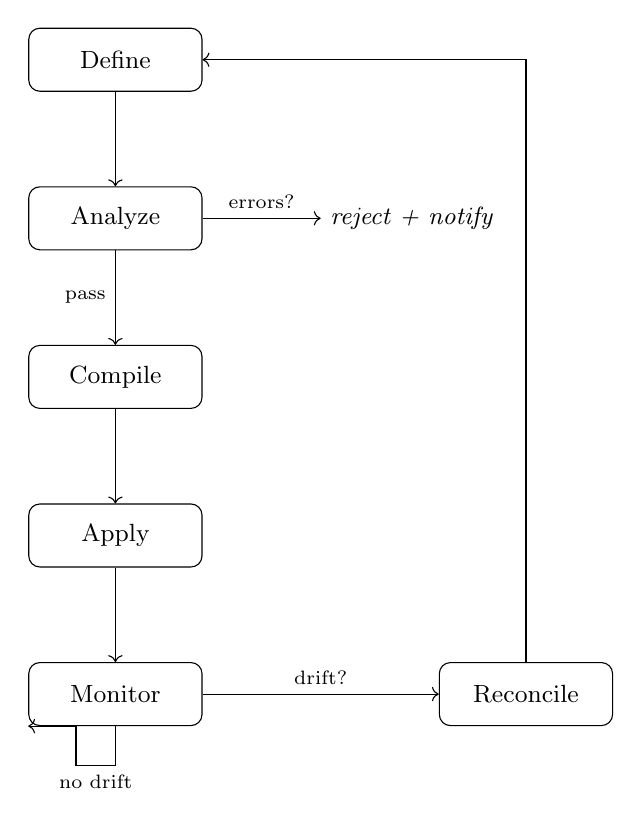
\begin{tikzpicture}[
  phase/.style={rectangle, draw, rounded corners, minimum width=2.2cm,
    minimum height=0.8cm, align=center, font=\small},
  every edge/.style={draw, -{Stealth[length=5pt]}},
  node distance=1.2cm,
]
  \node[phase] (define)    {Define};
  \node[phase, below=of define]    (analyze)   {Analyze};
  \node[phase, below=of analyze]   (compile)   {Compile};
  \node[phase, below=of compile]   (apply)     {Apply};
  \node[phase, below=of apply]     (monitor)   {Monitor};
  \node[phase, right=3cm of monitor] (reconcile) {Reconcile};
  \node[right=1.5cm of analyze, font=\small\itshape] (reject) {reject + notify};

  \draw[->] (define) -- (analyze);
  \draw[->] (analyze) -- node[left,font=\scriptsize]{pass} (compile);
  \draw[->] (analyze) -- node[above,font=\scriptsize]{errors?} (reject);
  \draw[->] (compile) -- (apply);
  \draw[->] (apply) -- (monitor);
  \draw[->] (monitor) -- node[above,font=\scriptsize]{drift?} (reconcile);
  \draw[->] (monitor.south) -- ++(0,-0.5) -| node[near start,below,font=\scriptsize]{no drift} ++(-0.5,0) |- (monitor.south west);
  \draw[->] (reconcile) |- (define);
\end{tikzpicture}
\caption{The six-phase governance loop: Define $\to$ Analyze $\to$ Compile $\to$
Apply $\to$ Monitor $\to$ Reconcile.}
\label{fig:governance-loop}
\end{figure}

\begin{enumerate}
  \item \textbf{Define}: Data stewards author policies using the DSL (atoms,
    clauses, selectors, traversals). Policies are version-controlled.
  \item \textbf{Analyze}: The analysis engine (Section~\ref{sec:analysis})
    validates all policies: satisfiability, contradiction detection, redundancy
    identification, and tenant isolation proofs. If errors are found, the
    policy set is rejected and authors are notified.
  \item \textbf{Compile}: Validated policies are compiled
    (Section~\ref{sec:compilation}) to PostgreSQL artifacts. The output is
    deterministic and reproducible.
  \item \textbf{Apply}: Compiled SQL statements are executed against the target
    database in a transaction.
  \item \textbf{Monitor}: The drift detection engine (Section~\ref{sec:drift})
    periodically introspects the database and compares observed state to
    expected state.
  \item \textbf{Reconcile}: When drift is detected, the reconciliation engine
    applies the appropriate strategy (auto-remediate, alert, or quarantine) and
    feeds findings back into the Define phase.
\end{enumerate}

\subsection{Governance State Machine}

\begin{definition}[Governance state]
\label{def:governance-state}
A governance state is a pair:
\[
G = (S, D)
\]
Where $S$ is the current policy set and $D$ is the current database state
(the observed state from Section~\ref{sec:drift}).
\end{definition}

\begin{definition}[Governance transitions]
\label{def:governance-transitions}
The governance loop defines transitions:
\begin{align*}
\mathrm{define}    &: (S, D) \to (S', D) \\
\mathrm{analyze}   &: (S, D) \to (S, D) \mid \mathit{error} \\
\mathrm{compile}   &: (S, D) \to (S, D, E) \\
\mathrm{apply}     &: (S, D, E) \to (S, D') \\
\mathrm{monitor}   &: (S, D) \to (S, D, \Delta) \\
\mathrm{reconcile} &: (S, D, \Delta) \to (S, D')
\end{align*}
\end{definition}

\subsection{Convergence}

\begin{property}[Convergence]
\label{prop:convergence}
Absent external changes to the database, one complete cycle of the governance
loop brings drift to zero:
\[
\mathrm{drift}(\mathrm{apply}(\mathrm{compile}(\mathrm{analyze}(S))), S) = \emptyset
\]
\end{property}

\begin{proof}[Sketch]
The \texttt{compile} function produces expected state $E$ from policy set $S$.
The \texttt{apply} function executes $E$ against the database, making observed
state $O$ equal to $E$. The \texttt{monitor} function computes
$O \mathbin{\triangle} E$, which is $E \mathbin{\triangle} E = \emptyset$.
\end{proof}

The ``absent external changes'' caveat is essential: another actor (DBA,
migration script, another tool) may modify the database between
\texttt{apply} and \texttt{monitor}, introducing drift that requires another cycle.

\subsection{Idempotence}

\begin{property}[Idempotence]
\label{prop:apply-idempotence}
Applying the same compiled artifacts twice produces the same database state:
\[
\mathrm{apply}(E, \mathrm{apply}(E, D)) = \mathrm{apply}(E, D)
\]
\end{property}

\begin{proof}[Sketch]
Each compiled artifact is a \texttt{CREATE POLICY \ldots\ IF NOT EXISTS} or an
idempotent \texttt{ALTER TABLE \ldots\ ENABLE ROW LEVEL SECURITY}. Re-executing
these statements on a database already in the target state is a no-op. For
\texttt{CREATE POLICY} without \texttt{IF NOT EXISTS}, the engine uses
\texttt{DROP POLICY IF EXISTS} followed by \texttt{CREATE POLICY}, which is
idempotent by construction.
\end{proof}

\subsection{Key Invariants}

The governance loop maintains the following invariants at steady state (zero drift):
\begin{enumerate}
  \item \textbf{RLS enabled}: Every governed table has $\texttt{relrowsecurity} = \texttt{true}$.
  \item \textbf{RLS forced}: Every governed table has $\texttt{relforcerowsecurity} = \texttt{true}$.
  \item \textbf{Policy match}: For every governed table $T$, the set of policies on $T$
    matches the compiled output of the policy set.
  \item \textbf{Grant match}: For every governed table $T$, the grants on $T$ match the
    compiled output.
  \item \textbf{Tenant isolation}: For every governed table $T$ that is subject to a
    tenant isolation policy, the isolation proof (Section~\ref{sec:analysis}) holds.
\end{enumerate}

% ============================================================
\section{Complete BNF Grammar}
\label{sec:bnf}
% ============================================================

This section assembles all grammar fragments from
Sections~\ref{sec:atoms}--\ref{sec:traversal} into a standalone grammar for
the policy algebra DSL.

\begin{lstlisting}[style=bnf]
(* ============================================== *)
(* Policy Algebra DSL -- Complete BNF Grammar      *)
(* ============================================== *)

(* --- Top Level --- *)

<policy_set>      ::= <policy>*

<policy>          ::= "POLICY" <identifier>
                      <policy_type>
                      <command_list>
                      <selector_clause>
                      <clause_block>

<policy_type>     ::= "PERMISSIVE" | "RESTRICTIVE"
<command_list>    ::= "FOR" <command> ("," <command>)*
<command>         ::= "SELECT" | "INSERT"
                    | "UPDATE" | "DELETE"
<selector_clause> ::= "SELECTOR" <selector>

(* --- Selectors --- *)

<selector>        ::= <base_selector>
                     | <selector> "AND" <selector>
                     | <selector> "OR" <selector>
                     | "NOT" <selector>
                     | "(" <selector> ")"
                     | "ALL"

<base_selector>   ::= "has_column(" <identifier>
                       ("," <type>)? ")"
                     | "in_schema(" <identifier> ")"
                     | "named(" <pattern> ")"
                     | "tagged(" <tag> ")"

(* --- Clauses --- *)

<clause_block>    ::= "CLAUSE" <clause>
                      ("OR" "CLAUSE" <clause>)*
<clause>          ::= <atom> ("AND" <atom>)*

(* --- Atoms --- *)

<atom>            ::= <value_source> <binary_op>
                      <value_source>
                    | <value_source> <unary_op>
                    | <traversal_atom>

<traversal_atom>  ::= "exists(" <relationship> ","
                      <clause> ")"

<relationship>    ::= "rel(" <identifier> ","
                      <identifier> "," <identifier> ","
                      <identifier> ")"

(* --- Value Sources --- *)

<value_source>    ::= "col(" <identifier> ")"
                    | "session(" <string_literal> ")"
                    | "lit(" <literal_value> ")"
                    | "fn(" <identifier> ","
                      "[" <arg_list>? "]" ")"

<arg_list>        ::= <value_source>
                      ("," <value_source>)*

(* --- Operators --- *)

<binary_op>       ::= "=" | "!=" | "<" | ">" | "<="
                     | ">=" | "IN" | "NOT IN"
                     | "LIKE" | "NOT LIKE"

<unary_op>        ::= "IS NULL" | "IS NOT NULL"

(* --- Literals and Identifiers --- *)

<literal_value>   ::= <string_literal>
                     | <integer_literal>
                     | <boolean_literal>
                     | <null_literal>
                     | <list_literal>

<list_literal>    ::= "[" <literal_value>
                      ("," <literal_value>)* "]"

<string_literal>  ::= "'" <character>* "'"
<integer_literal> ::= ["-"] <digit>+
<boolean_literal> ::= "true" | "false"
<null_literal>    ::= "null"

<identifier>      ::= <letter>
                      (<letter> | <digit> | "_")*

<pattern>         ::= <string_literal>
<tag>             ::= <string_literal>

<type>            ::= "text" | "integer" | "bigint"
                     | "uuid" | "boolean" | "timestamp"
                     | "jsonb"
\end{lstlisting}

% ============================================================
\section{Summary of Properties \& Lemmas}
\label{sec:summary}
% ============================================================

Table~\ref{tab:summary} lists all theorems, properties, and lemmas established
in this specification.

\begin{table*}[t]
\caption{Summary of properties and lemmas}
\label{tab:summary}
\centering
\small
\begin{tabular}{llll}
\toprule
\# & Name & Statement & Section \\
\midrule
T1.1  & Undecidability of arbitrary RLS
      & Row accessibility under arbitrary SQL RLS predicates is undecidable
      & \ref{sec:introduction} \\
P2.1  & Decidability of atom satisfiability
      & Satisfiability of any finite conjunction of atoms is decidable
      & \ref{sec:atoms} \\
P3.1  & Clause satisfiability
      & A normalized clause is satisfiable iff $c \neq \bot$
      & \ref{sec:clauses} \\
P3.2  & Clause subsumption
      & $c_1 \subseteq c_2$ implies $\denote{c_2} \subseteq \denote{c_1}$
      & \ref{sec:clauses} \\
P3.3  & Idempotence
      & $c \land c = c$ for any clause $c$
      & \ref{sec:clauses} \\
P5.1  & Monotonicity of permissive extension
      & Adding a permissive policy can only increase accessible rows
      & \ref{sec:composition} \\
P5.2  & Anti-monotonicity of restrictive extension
      & Adding a restrictive policy can only decrease accessible rows
      & \ref{sec:composition} \\
L5.1  & Subsumed permissive redundancy
      & A permissive policy subsumed by another is redundant
      & \ref{sec:composition} \\
P6.1  & Selector monotonicity
      & Adding tables preserves existing selector matches
      & \ref{sec:selectors} \\
P7.1  & Bounded compilation
      & Traversal depth $d$ $\to$ at most $d$ nested EXISTS
      & \ref{sec:traversal} \\
P7.2  & No recursive traversal
      & Hierarchies require closure tables
      & \ref{sec:traversal} \\
T8.1  & Tenant isolation sufficient condition
      & If every permissive clause has the tenant atom, isolation holds
      & \ref{sec:analysis} \\
P9.1  & Termination of normalization
      & Normalization terminates (strict reduction under lex ordering)
      & \ref{sec:optimization} \\
P9.2  & Correctness of normalization
      & Each rewrite rule preserves denotation
      & \ref{sec:optimization} \\
T10.1 & Compilation correctness
      & Accessible rows under SQL $=$ rows satisfying $\Eff(T, \CMD)$
      & \ref{sec:compilation} \\
P10.1 & Monotonicity of compilation
      & Subsumption in DSL preserved in compiled SQL
      & \ref{sec:compilation} \\
P10.2 & Determinism of compilation
      & Same normal form $\to$ identical SQL output
      & \ref{sec:compilation} \\
P12.1 & Convergence
      & One governance cycle brings drift to zero
      & \ref{sec:governance-loop} \\
P12.2 & Idempotence of application
      & Applying same artifacts twice $=$ same state
      & \ref{sec:governance-loop} \\
\bottomrule
\end{tabular}
\end{table*}

% ============================================================
\appendix
% ============================================================

\section{Full Lifecycle Worked Example}
\label{app:worked-example}

This appendix traces the complete governance lifecycle for our running example
schema, exercising every definition in the specification.

\subsection{Define}

We define three policies:

\begin{lstlisting}[style=dsl]
POLICY tenant_isolation
  PERMISSIVE
  FOR SELECT, INSERT, UPDATE, DELETE
  SELECTOR has_column('tenant_id')
  CLAUSE col('tenant_id') = session('app.tenant_id')

POLICY tenant_isolation_via_project
  PERMISSIVE
  FOR SELECT, INSERT, UPDATE, DELETE
  SELECTOR named('tasks') OR named('files')
  CLAUSE
    exists(
      rel(_, project_id, projects, id),
      {col('tenant_id') = session('app.tenant_id')}
    )

POLICY soft_delete
  RESTRICTIVE
  FOR SELECT
  SELECTOR has_column('is_deleted')
  CLAUSE col('is_deleted') = lit(false)
\end{lstlisting}

\subsection{Selector Evaluation}

Evaluate selectors against the running example metadata:

\begin{table}[h]
\centering
\begin{tabular}{ll}
\toprule
Selector & Matching tables \\
\midrule
\texttt{has\_column('tenant\_id')} & users, projects, comments \\
\texttt{named('tasks') OR named('files')} & tasks, files \\
\texttt{has\_column('is\_deleted')} & projects \\
\bottomrule
\end{tabular}
\end{table}

Policy-to-table mapping:

\begin{table}[h]
\centering
\begin{tabular}{ll}
\toprule
Table & Policies applied \\
\midrule
users    & tenant\_isolation \\
projects & tenant\_isolation, soft\_delete \\
tasks    & tenant\_isolation\_via\_project \\
comments & tenant\_isolation \\
files    & tenant\_isolation\_via\_project \\
config   & \emph{(none --- default deny)} \\
\bottomrule
\end{tabular}
\end{table}

\subsection{Normalize}

All three policies are already in normal form:
\begin{itemize}
  \item Each clause has one atom, in atom normal form.
  \item No unsatisfiable clauses.
  \item No subsumption between clauses within the same policy.
\end{itemize}

\subsection{Analyze}

\subsubsection{Satisfiability}

\begin{itemize}
  \item \texttt{tenant\_isolation} clause:
    $\texttt{col('tenant\_id')} = \texttt{session('app.tenant\_id')}$ ---
    satisfiable (session variable can equal any \texttt{tenant\_id} value).
  \item \texttt{tenant\_isolation\_via\_project} clause:
    $\texttt{exists}(\texttt{rel}(\ldots), \ldots)$ --- satisfiable (there can
    exist a matching project row).
  \item \texttt{soft\_delete} clause:
    $\texttt{col('is\_deleted')} = \texttt{lit(false)}$ --- satisfiable.
\end{itemize}

All clauses pass satisfiability.

\subsubsection{Contradiction Check}

For \texttt{projects} (SELECT):
\[
\Eff(\texttt{projects}, \texttt{SELECT}) =
(\texttt{col('tenant\_id')} = \texttt{session('app.tenant\_id')})
\land (\texttt{col('is\_deleted')} = \texttt{lit(false)})
\]

SMT encoding: $\mathit{tid\_var} = \mathit{session\_tid} \land \mathit{is\_deleted\_var} = \mathit{false}$.
Satisfiable. No contradiction.

\subsubsection{Tenant Isolation Proof}

\begin{itemize}
  \item For \texttt{users}: The sole permissive clause contains
    $\texttt{col('tenant\_id')} = \texttt{session('app.tenant\_id')}$.
    By Theorem~\ref{thm:tenant-isolation}, isolation holds.
  \item For \texttt{projects}: Same as \texttt{users}.
  \item For \texttt{tasks}: The permissive clause uses traversal to check
    \texttt{tenant\_id} on \texttt{projects}. By the extended form of
    Theorem~\ref{thm:tenant-isolation} (depth-1 traversal), isolation holds.
  \item For \texttt{comments}: Same as \texttt{users}.
  \item For \texttt{files}: Same reasoning as \texttt{tasks}.
  \item For \texttt{config}: No permissive policies $\to$ default deny $\to$
    no access at all $\to$ isolation trivially holds.
\end{itemize}

\textbf{Result}: Tenant isolation proven for all tables.

\subsection{Compile}

Generated SQL for each governed table:

\begin{lstlisting}[style=sql]
-- ====================================
-- users
-- ====================================
ALTER TABLE public.users
  ENABLE ROW LEVEL SECURITY;
ALTER TABLE public.users
  FORCE ROW LEVEL SECURITY;

CREATE POLICY tenant_isolation_users
  ON public.users
  AS PERMISSIVE
  FOR SELECT, INSERT, UPDATE, DELETE
  USING (tenant_id =
    current_setting('app.tenant_id'));

-- ====================================
-- projects
-- ====================================
ALTER TABLE public.projects
  ENABLE ROW LEVEL SECURITY;
ALTER TABLE public.projects
  FORCE ROW LEVEL SECURITY;

CREATE POLICY tenant_isolation_projects
  ON public.projects
  AS PERMISSIVE
  FOR SELECT, INSERT, UPDATE, DELETE
  USING (tenant_id =
    current_setting('app.tenant_id'));

CREATE POLICY soft_delete_projects
  ON public.projects
  AS RESTRICTIVE
  FOR SELECT
  USING (is_deleted = false);

-- ====================================
-- tasks
-- ====================================
ALTER TABLE public.tasks
  ENABLE ROW LEVEL SECURITY;
ALTER TABLE public.tasks
  FORCE ROW LEVEL SECURITY;

CREATE POLICY tenant_isolation_via_project_tasks
  ON public.tasks
  AS PERMISSIVE
  FOR SELECT, INSERT, UPDATE, DELETE
  USING (EXISTS (
    SELECT 1 FROM public.projects
    WHERE public.projects.id
          = public.tasks.project_id
      AND public.projects.tenant_id
          = current_setting('app.tenant_id')
  ));

-- ====================================
-- comments
-- ====================================
ALTER TABLE public.comments
  ENABLE ROW LEVEL SECURITY;
ALTER TABLE public.comments
  FORCE ROW LEVEL SECURITY;

CREATE POLICY tenant_isolation_comments
  ON public.comments
  AS PERMISSIVE
  FOR SELECT, INSERT, UPDATE, DELETE
  USING (tenant_id =
    current_setting('app.tenant_id'));

-- ====================================
-- files
-- ====================================
ALTER TABLE public.files
  ENABLE ROW LEVEL SECURITY;
ALTER TABLE public.files
  FORCE ROW LEVEL SECURITY;

CREATE POLICY tenant_isolation_via_project_files
  ON public.files
  AS PERMISSIVE
  FOR SELECT, INSERT, UPDATE, DELETE
  USING (EXISTS (
    SELECT 1 FROM public.projects
    WHERE public.projects.id
          = public.files.project_id
      AND public.projects.tenant_id
          = current_setting('app.tenant_id')
  ));
\end{lstlisting}

\subsection{Apply}

Execute the compiled SQL in a transaction against the target PostgreSQL
database. All statements succeed.

\subsection{Simulate Drift}

A DBA manually runs:

\begin{lstlisting}[style=sql]
ALTER TABLE public.projects
  DISABLE ROW LEVEL SECURITY;

CREATE POLICY manual_override ON public.users
  AS PERMISSIVE FOR SELECT
  USING (true);
\end{lstlisting}

This introduces two drift items:
\begin{enumerate}
  \item RLS disabled on \texttt{projects}
  \item Extra (unmanaged) policy on \texttt{users}
\end{enumerate}

\subsection{Detect}

The drift detection algorithm (Section~\ref{sec:drift}) runs:

\begin{lstlisting}[style=pseudo]
detect_drift(S, {users, projects, tasks,
                 comments, files}) ->
{
    DriftItem(projects, "rls_disabled"),
    DriftItem(users, "extra_policy",
              "manual_override")
}
\end{lstlisting}

\subsection{Reconcile}

\begin{itemize}
  \item \texttt{projects} / \texttt{rls\_disabled} $\to$
    \textbf{auto-remediate}: re-enable RLS.
  \item \texttt{users} / \texttt{extra\_policy} $\to$ \textbf{alert}: notify
    operators about unmanaged policy \texttt{manual\_override}.
\end{itemize}

Remediation SQL:
\begin{lstlisting}[style=sql]
ALTER TABLE public.projects
  ENABLE ROW LEVEL SECURITY;
\end{lstlisting}

After remediation, the next monitoring cycle detects zero drift (assuming the
\texttt{extra\_policy} alert has been acknowledged or the manual policy has
been reviewed and either adopted into the policy set or dropped).

% ============================================================
\section{Glossary}
\label{app:glossary}
% ============================================================

\begin{description}
  \item[Atom] An irreducible boolean comparison:
    $(\mathit{left\_source}, \mathit{operator}, \mathit{right\_source})$.
    The smallest unit of the policy algebra.
  \item[Clause] A conjunction (AND) of atoms. Represents a single access
    condition that must be fully satisfied.
  \item[Compilation] The deterministic translation of a policy set to
    PostgreSQL SQL artifacts.
  \item[Default deny] The principle that if no permissive policy grants access,
    no rows are accessible.
  \item[Denotation] The semantic interpretation $\denote{\cdot}$ of a policy
    expression: the set of rows it matches.
  \item[Drift] Any discrepancy between the observed database state and the
    expected state derived from the policy algebra.
  \item[Effective access predicate] The combined predicate
    $(\bigvee\text{ permissive}) \land (\bigwedge\text{ restrictive})$ that
    determines row accessibility.
  \item[FCA] Formal Concept Analysis. A mathematical framework for deriving
    concept hierarchies from object-attribute relations.
  \item[Galois connection] A pair of monotone functions between ordered sets
    satisfying an adjunction property. Used to relate DSL and SQL semantics.
  \item[Governance loop] The six-phase cycle:
    Define $\to$ Analyze $\to$ Compile $\to$ Apply $\to$ Monitor $\to$ Reconcile.
  \item[Normalization] The process of applying rewrite rules to reduce a policy
    to its canonical form.
  \item[Permissive policy] A policy whose clauses are OR'd together with other
    permissive policies. Grants access.
  \item[Policy] A named, typed collection of clauses with a selector and
    command set.
  \item[Policy set] The complete collection of policies governing a database.
  \item[Reconciliation] The process of resolving drift between observed and
    expected database state.
  \item[Relationship] A declared foreign-key link between tables, used for
    traversal atoms.
  \item[Restrictive policy] A policy whose clauses are AND'd with the
    permissive disjunction. Narrows access.
  \item[RLS] Row-Level Security. PostgreSQL's mechanism for attaching
    row-filtering predicates to tables.
  \item[Selector] A predicate over table metadata that determines which tables
    a policy applies to.
  \item[SMT] Satisfiability Modulo Theories. A decision procedure for logical
    formulas over combined theories.
  \item[Subsumption] Relation where one policy/clause is at least as permissive
    as another.
  \item[Traversal atom] An atom that uses
    $\texttt{exists}(\mathit{relationship}, \mathit{clause})$ to follow a
    foreign-key relationship.
  \item[Value source] A typed scalar producer: column reference, session
    variable, literal, or function call.
\end{description}

% ============================================================
% Bibliography
% ============================================================

\nocite{zanzibar2019}  % Listed in original spec references
\bibliographystyle{ACM-Reference-Format}
\bibliography{references}

\end{document}
